\section{代码执行位置}
并行编程并不是真正意义上的快车道行驶。 它实际上是在所有车道上快速行驶。 本章的主题是让我们能够将代码放在尽可能多的地方。 
只要有意义,我们就会选择启用异构系统中的所有计算资源。 
因此,我们需要知道这些计算资源隐藏在哪里(找到它们)并使它们发挥作用(在它们上执行我们的代码)。

我们可以控制代码的执行位置,换句话说,我们可以控制哪些设备用于哪些Kernel。 
带有 SYCL 的 C++ 提供了异构编程框架,其中代码可以在主机 CPU 和设备的混合上执行。 
确定代码执行位置的机制对于我们理解和使用非常重要。

本章描述代码可以在哪里执行、何时执行以及用于控制执行位置的机制。 
第 3 章将描述如何管理数据,以便数据到达我们执行代码的地方,然后第 4 章返回代码本身并讨论Kernel的编写。


\subsection{单源}
\begin{figure}[H]
	\centering
	
\includegraphics[width=0.9\textwidth]{figs/F2.1.png}
	\caption{\textit{单源代码包含主机代码(在 CPU 上运行)和设备代码(在 SYCL 设备上运行)}}
\end{figure}


\begin{figure}[H]
	\centering
	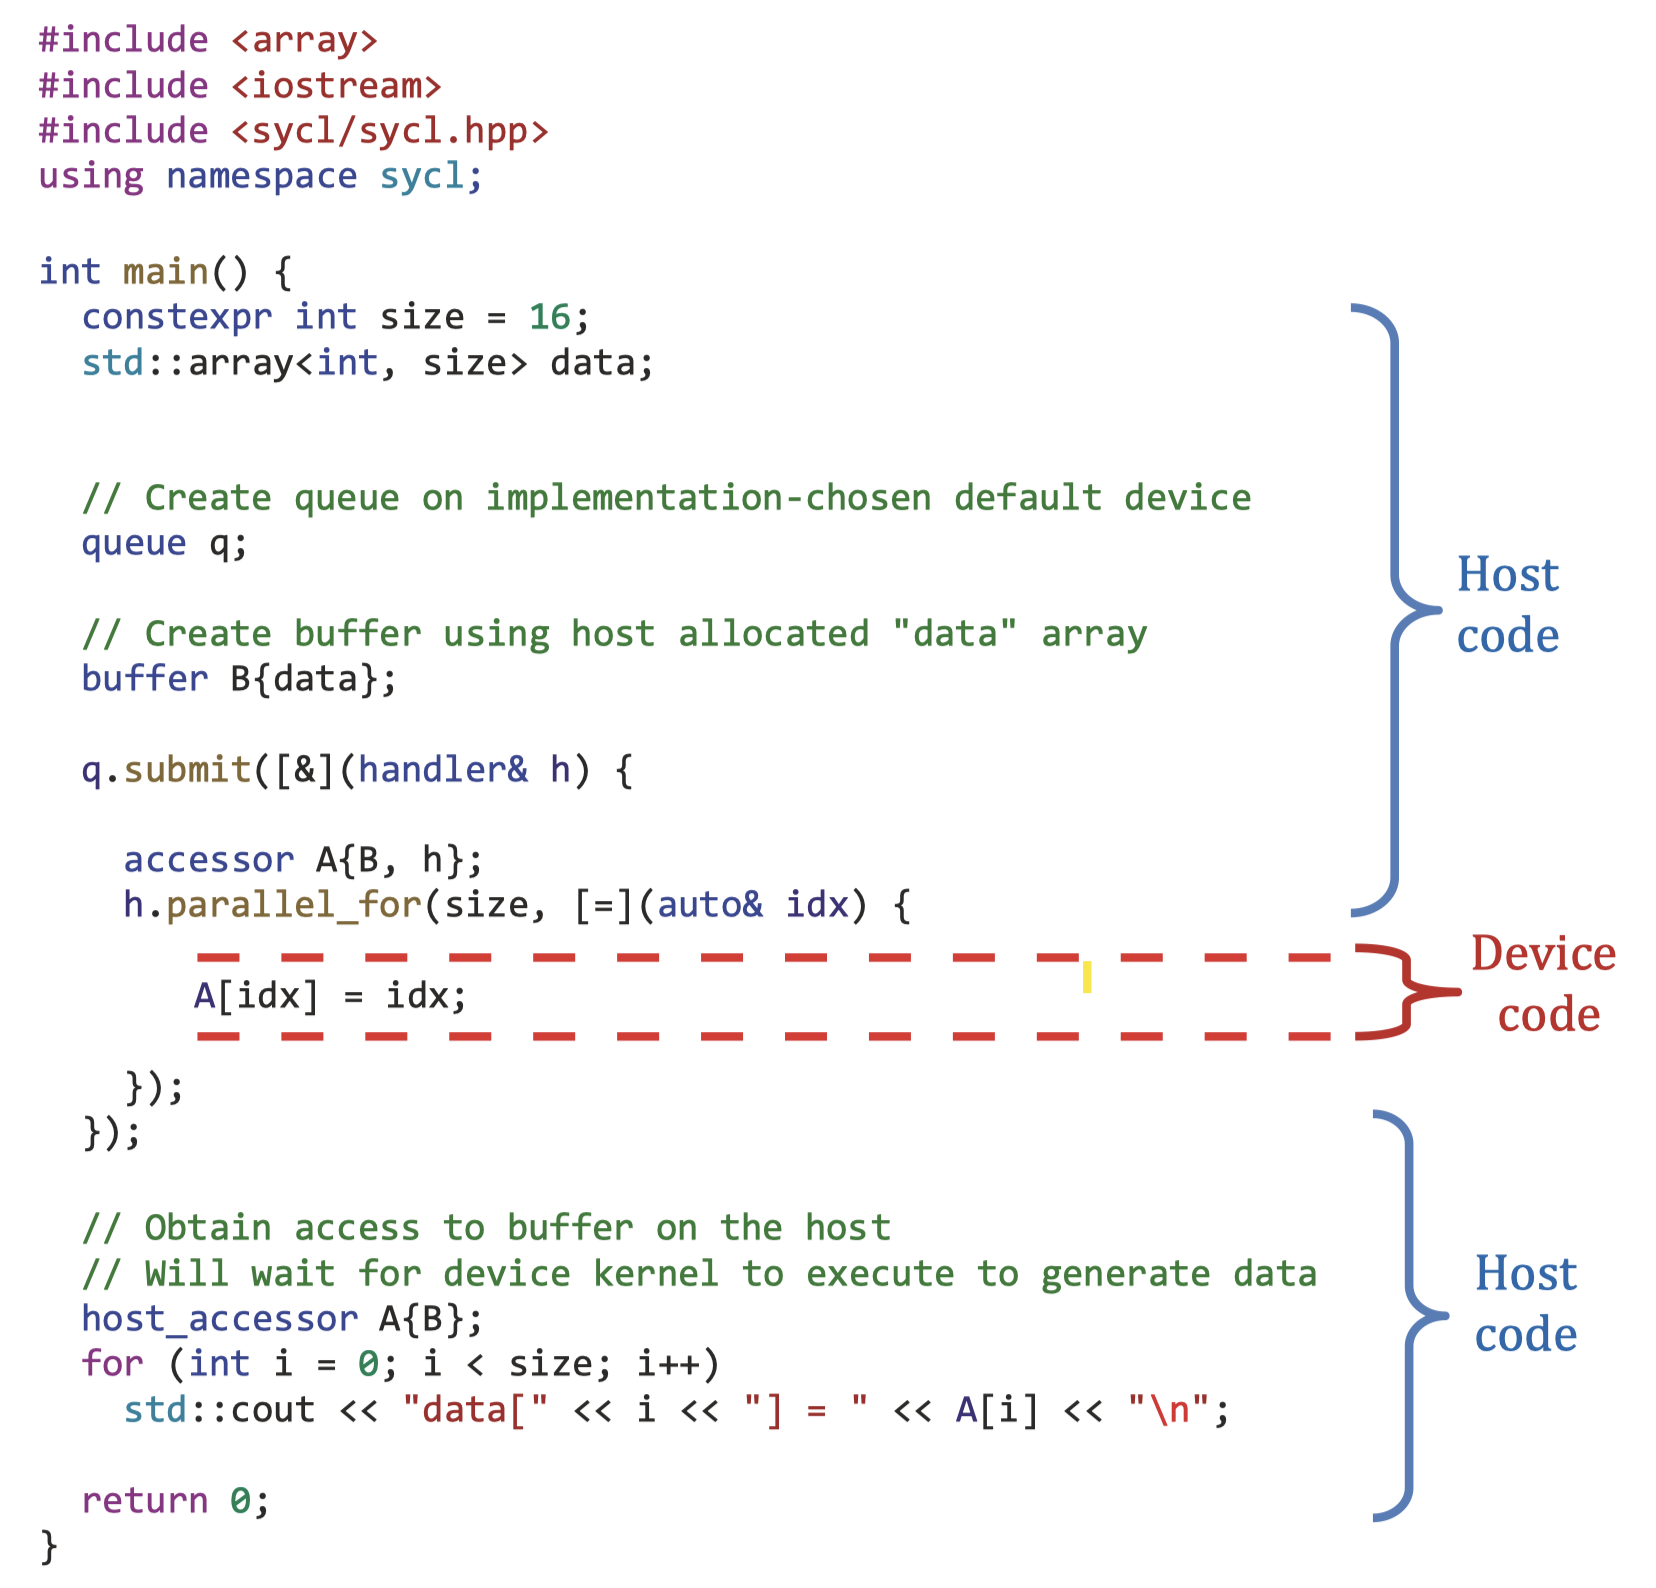
\includegraphics[width=0.9\textwidth]{figs/F2.2.png}
	\caption{\textit{简单的SYCL程序}}
\end{figure}

带有 SYCL 程序的 C++ 是单源的,这意味着相同的翻译单元(通常是源文件及其标头)
既包含定义要在 SYCL 设备上执行的计算Kernel的代码,也包含协调这些Kernel执行的主机代码 。 
图 2-1 以图形方式显示了这两个代码路径,图 2-2 提供了一个示例应用程序,其中标记了主机和设备代码区域。

将设备和主机代码组合到单个源文件(或翻译单元)中可以使异构应用程序更容易理解和维护。 
该组合还提供了改进的语言类型安全性,并且可以导致我们的代码的更多编译器优化。

\subsubsection{主机代码}
应用程序包含 C++ 主机代码,由动作系统在其上启动应用程序的 CPU 执行。 
主机代码是应用程序的主干,它定义和控制可用设备的工作分配。 它也是我们定义应由 SYCL 运行时管理的数据和依赖项的接口。

主机代码是标准 C++,并添加了可作为 C++ 库实现的 SYCL 特定构造和类。 
这使得更容易推断主机代码中允许的内容(C++ 中允许的任何内容),并且可以简化与构建系统的集成。

应用程序中的主机代码协调数据移动和计算卸载到设备,但也可以自行执行计算密集型工作,
并且可以像任何 C++ 应用程序一样使用库。

\subsubsection{设备代码}
设备对应于概念上独立于执行主机代码的CPU 的加速器或处理器。 实现也可以将主机处理器公开为设备,如本章后面所述,
但主机处理器和设备应该被认为在逻辑上彼此独立。 
主机处理器运行本机 C++ 代码,而设备运行包含一些附加功能和限制的设备代码。

队列是一种将工作提交到设备以供将来执行的机制。 需要了解设备代码的三个重要属性:

\begin{enumerate}
	\item \textbf{它从主机代码异步执行。} 主机程序向设备提交设备代码,只有当所有执行依赖性都得到满足时,
	运行时才会跟踪并启动该工作(更多内容将在第 3 章中介绍)。 
	主机程序执行在设备上启动提交的工作之前进行,从而提供了设备上的执行与主机程序执行异步的属性,
	除非我们明确地将两者绑定在一起。 作为这种异步执行的副作用,
	只有主机程序通过我们在后面的章节中介绍的各种机制(例如主机访问器和阻塞队列等待动作)强制执行开始,
	才能保证设备上的工作开始。

	\item \textbf{对设备代码进行限制} ,使其能够在加速器设备上编译并实现性能。 
	例如,设备代码中不支持动态内存分配和运行时类型信息 (RTTI),因为它们会导致许多加速器的性能下降。 
	第 10 章详细介绍了一小部分设备代码限制。

	\item \textbf{SYCL 定义的一些函数和查询仅在设备代码中可用} ,因为它们只在那里有意义,
	例如,工作项标识符查询允许设备代码的执行实例查询其在更大的数据并行范围中的位置(描述 第 4 章)。
\end{enumerate}

一般来说,我们将提交到队列的工作称为动作。 
动作包括在设备上执行设备代码,但在第 3 章中我们将了解到动作还包括内存移动命令。 
在本章中,由于我们关注动作的设备代码方面,因此我们将在大部分时间中具体提及设备代码。

\subsection{选择设备}
为了探索让我们控制设备代码执行位置的机制,我们将看五个用例:

\textbf{方法\#1} :当我们不关心使用哪个设备时,在某个地方运行设备代码。 这通常是开发的第一步,因为它是最简单的。

\textbf{方法\#2} :在 CPU 设备上显式运行设备代码,通常用于调试,因为大多数开发系统都有可访问的 CPU。 
CPU 调试器通常也具有非常丰富的功能。

\textbf{方法\#3} :将设备代码分派到 GPU 或其他加速器。

\textbf{方法\#4} :将设备代码分派到一组异构设备,例如 GPU 和 FPGA。

\textbf{方法\#5} :从更通用的设备类别中选择特定设备,例如从可用 FPGA 类型集合中选择特定类型的 FPGA。

\begin{remark}
	开发人员通常会使用 Method\#2 尽可能多地调试代码,
	并且只有在使用 Method\#2 对代码进行了尽可能多的测试后才转向方法 \#3–\#5。
\end{remark}

\subsection{方法\#1:在任何类型的设备上运行}
当我们不关心设备代码将在哪里运行时,很容易让运行时为我们选择。 
这种自动选择的目的是让我们在不关心选择什么设备时可以轻松地开始编写和运行代码。 
此设备选择没有考虑要运行的代码,因此应被视为任意选择,可能不是最佳选择。

在讨论设备的选择之前,即使是实现为我们选择的设备,我们应该首先介绍程序与设备交互的机制:队列。

\subsubsection{队列}
\begin{figure}[H]
	\centering
	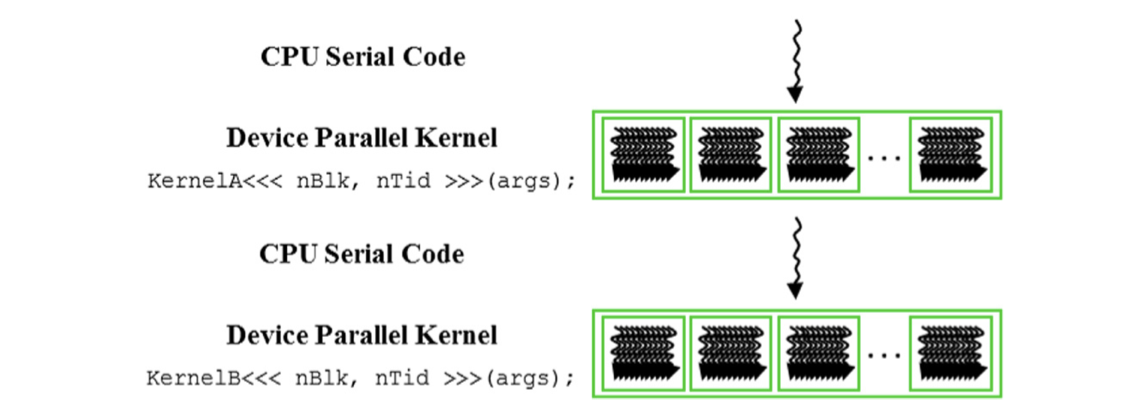
\includegraphics[width=0.9\textwidth]{figs/F2.3.png}
	\caption{\textit{队列类的某些构造函数的简化定义}}
\end{figure}

\begin{figure}[H]
	\centering
	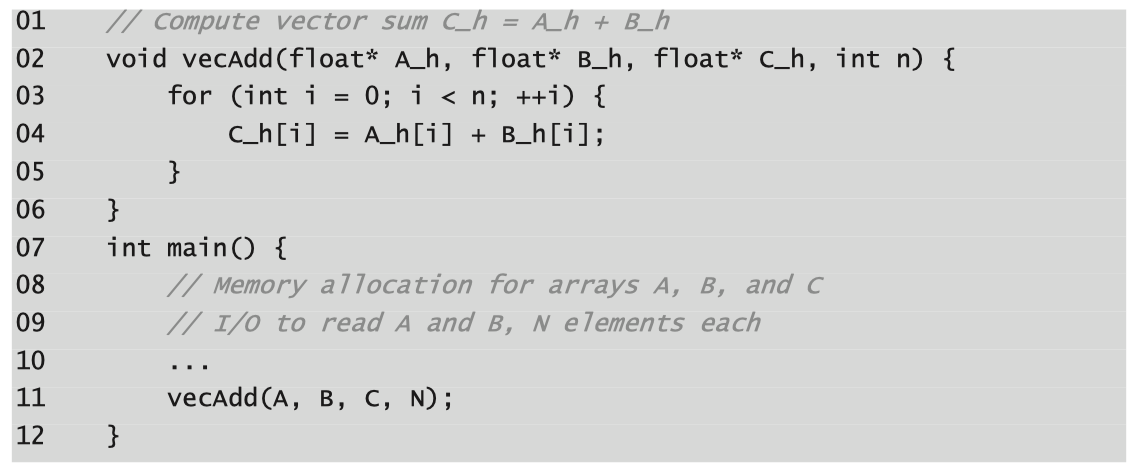
\includegraphics[width=0.9\textwidth]{figs/F2.4.png}
	\caption{\textit{简化了队列类中一些关键成员函数的定义}}
\end{figure}


队列是一个抽象概念,动作被提交到该抽象概念以便在单个设备上执行。 图 2-3 和 2-4 给出了队列类的简化定义。 
动作通常是数据并行计算的启动,尽管也可以使用其他命令,例如当我们需要比 SYCL 运行时提供的自动移动更多的控制时,
手动控制数据移动。 提交到队列的工作可以在满足运行时跟踪的先决条件(例如输入数据的可用性)后执行。 
第 3 章和第 8 章介绍了这些先决条件。

\begin{figure}[H]
	\centering
	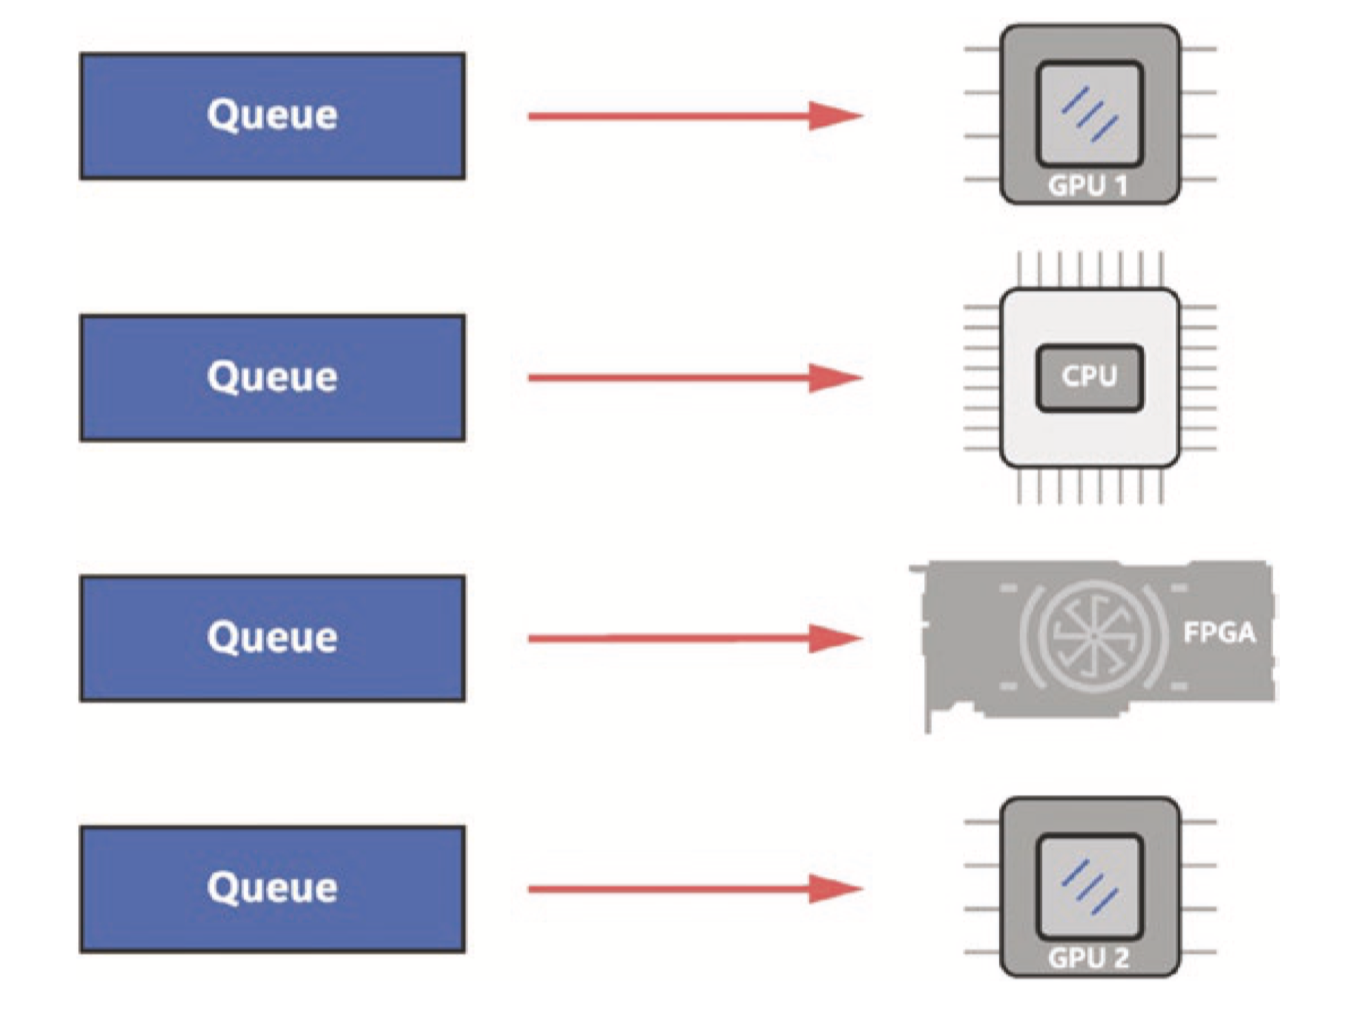
\includegraphics[width=0.9\textwidth]{figs/F2.5.png}
	\caption{\textit{队列绑定到单个设备。提交到队列的工作在该设备上执行}}
\end{figure}

队列绑定到单个设备,并且该绑定发生在队列的构造上。 重要的是要了解提交到队列的工作是在该队列绑定到的单个设备上执行的。 
队列无法映射到设备集合,因为这会导致哪个设备应执行工作不明确。 同样,队列无法将提交给它的工作分散到多个设备上。 
相反,队列与执行提交到该队列的工作的设备之间存在明确的映射,如图 2-5 所示。

\begin{figure}[H]
	\centering
	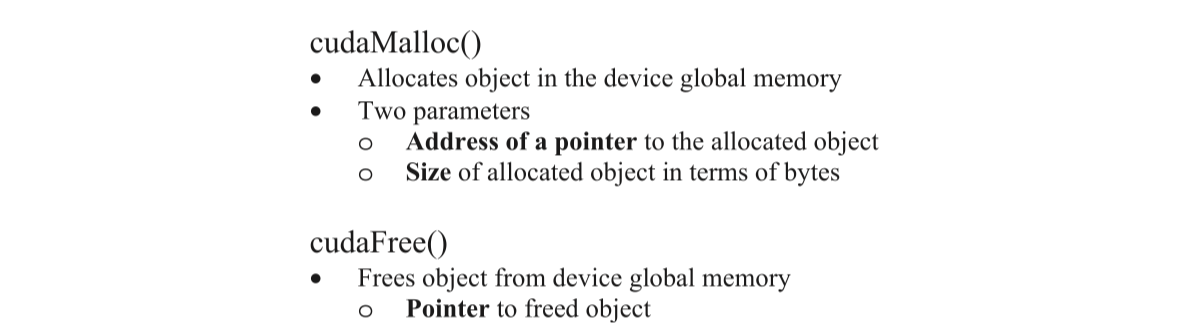
\includegraphics[width=0.9\textwidth]{figs/F2.6.png}
	\caption{\textit{多个队列可以绑定到单个设备}}
\end{figure}

可以按照我们希望的应用程序架构或编程风格的任何方式在程序中创建多个队列。 
例如,可以创建多个队列以分别与不同的设备绑定或由主机程序中的不同线程使用。 
多个不同的队列可以绑定到单个设备(例如 GPU),并且向这些不同队列的提交将导致在设备上执行组合工作。 
图 2-6 显示了一个示例。 相反,正如我们之前提到的,一个队列不能绑定到多个设备,因为请求执行动作的位置不能有任何歧义。 
例如,如果我们想要一个能够跨多个设备负载平衡工作的队列,那么我们可以在代码中创建该抽象。

由于队列绑定到特定设备,因此队列构造是代码中选择将执行提交到队列的动作的设备的最常见方法。 
构造队列时设备的选择是通过设备选择器抽象来实现的。

\subsubsection{当任何设备都可以时将队列绑定到设备}
\begin{figure}[H]
	\centering
	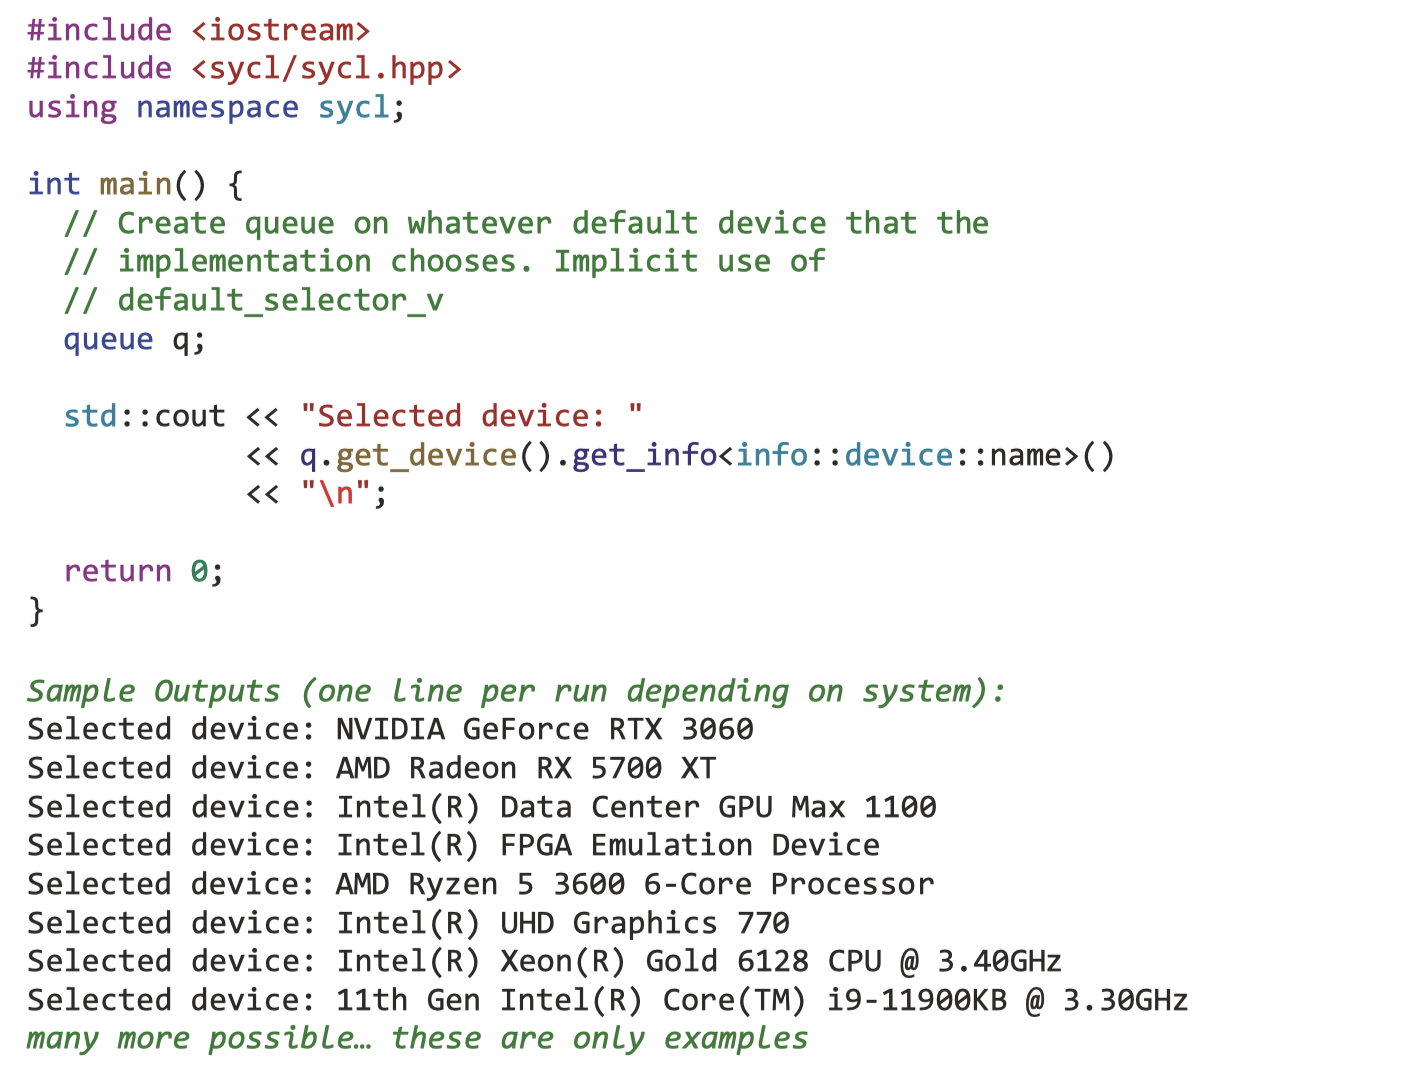
\includegraphics[width=0.9\textwidth]{figs/F2.7.png}
	\caption{\textit{通过队列的默认构造隐式默认设备选择器}}
\end{figure}

图 2-7 是未指定队列应绑定到的设备的示例。 不带任何参数的默认队列构造函数(如图 2-7 所示)只是在幕后选择一些可用的设备。 
SYCL 保证至少有一个设备始终可用,因此这种默认选择机制将始终选择某个设备。 
在许多情况下,所选设备可能恰好是也正在执行主机程序的CPU,尽管不能保证这一点。

使用简单的队列构造函数是开始应用程序开发以及启动和运行设备代码的简单方法。 
当它与我们的应用程序相关时,可以添加对绑定到队列的设备的选择的更多控制。

\subsection{方法\#2:使用 CPU 设备进行开发、调试和部署}
CPU 设备可以被认为使主机 CPU 能够像独立设备一样运行,从而允许我们的设备代码执行,而不管系统中是否有可用的加速器。 
我们总是有一些处理器运行主机程序,因此 CPU 设备通常可供我们的应用程序使用(极少数情况下,由于各种原因,
CPU 可能不会通过实现公开为 SYCL 设备)。 使用 CPU 设备进行代码开发有几个优点:

\begin{enumerate}
	\item 在没有任何加速器的功能较差的系统上开发设备代码:一种常见用途是在本地系统上开发和测试设备代码,
	然后部署到 HPC 集群进行性能测试和优化。

	\item 使用非加速器工具调试设备代码:加速器通常通过较低级别的 API 公开,
	这些 API 可能没有主机 CPU 可用的先进调试工具。 考虑到这一点,CPU 设备通常支持使用开发人员熟悉的标准工具进行调试。

	\item 如果没有其他设备可用,则进行备份,以保证设备代码可以正常执行:CPU 设备可能不以性能为主要目标,
	或者可能与Kernel代码优化的架构不匹配,但通常可以考虑 作为功能备份,以确保设备代码始终可以在任何应用程序中执行。
\end{enumerate}

发现 SYCL 应用程序可以使用多个 CPU 设备应该不足为奇,其中一些旨在简化调试,而另一些则可能专注于执行性能。 
设备方面可用于区分这些不同的 CPU 设备,如本章后面所述。

当考虑使用 CPU 设备来开发和调试设备代码时,应考虑 CPU 和目标加速器架构(例如 GPU)之间的差异。 
特别是在优化代码性能时,特别是在使用更高级的功能(例如子组)时,跨架构的功能和性能可能存在一些差异。 
例如,当移动到新设备时,子组大小可能会发生变化。 
大多数开发和调试通常可以在 CPU 设备上进行,有时随后在目标设备架构上进行最终调整和调试。

\begin{figure}[H]
	\centering
	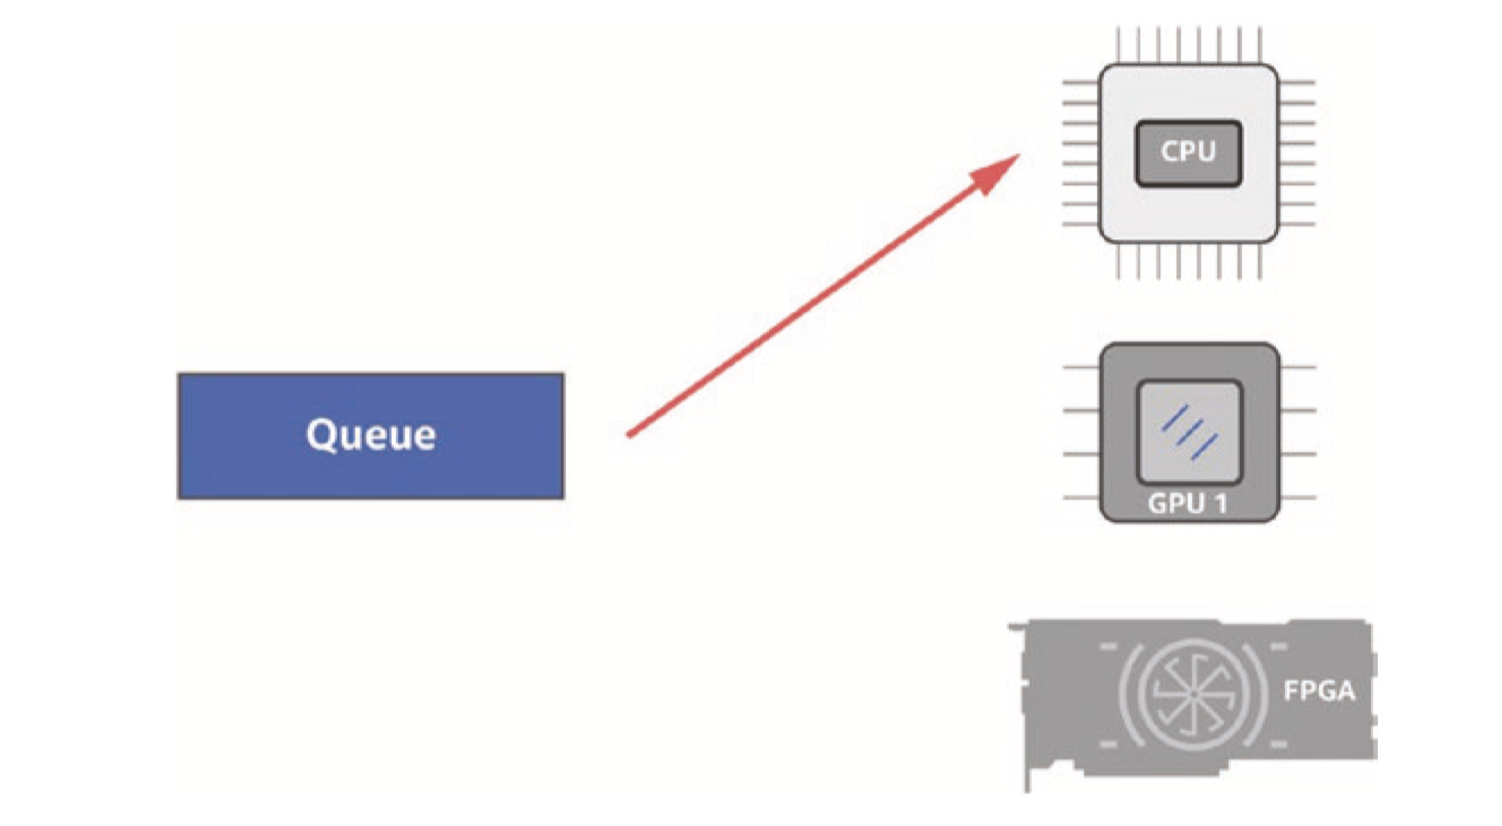
\includegraphics[width=0.9\textwidth]{figs/F2.8.png}
	\caption{\textit{CPU 设备可以像任何加速器一样执行设备代码}}
\end{figure}

CPU 设备在功能上类似于硬件加速器,队列可以与其绑定并且可以执行设备代码。 
图 2-8 显示了 CPU 设备如何与系统中可用的其他加速器对等。 
它可以执行设备代码,就像 GPU 或 FPGA 能够执行的方式一样,并且可以构建一个或多个与其绑定的队列。

\begin{figure}[H]
	\centering
	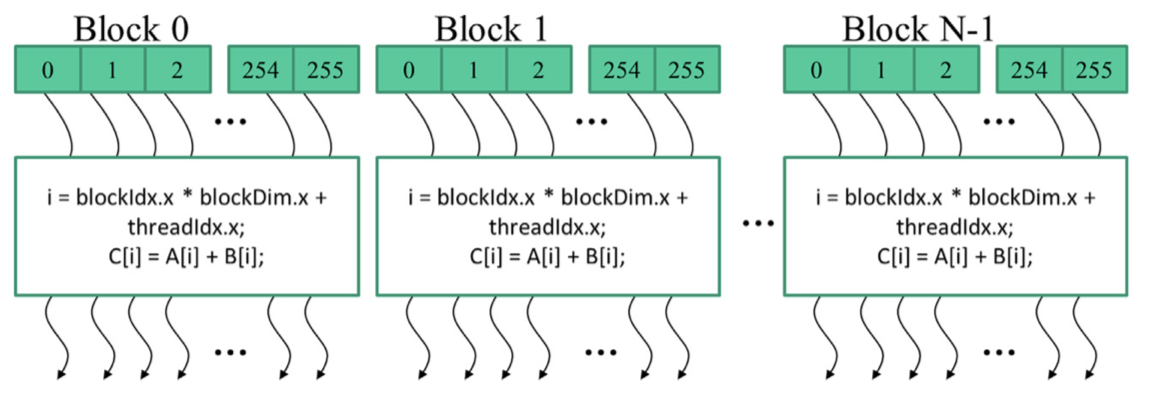
\includegraphics[width=0.9\textwidth]{figs/F2.9.png}
	\caption{\textit{使用 cpu\_selector\_v 选择主机设备}}
\end{figure}

应用程序可以通过将 cpu\_selector\_v 显式传递给队列构造函数来选择创建绑定到 CPU 设备的队列,如图 2-9 所示。

即使没有特别请求(例如,使用 cpu\_selector\_v),CPU 设备也可能恰好被默认选择器选择,如图 2-7 中的输出所示。

定义了设备选择器的一些变体,以便我们轻松地定位某种类型的设备。 
cpu\_selector\_v 是这些选择器的一个示例,我们将在接下来的部分中介绍其他选择器。

\subsection{方法\#3:使用 GPU(或其他加速器)}
下一个示例将展示 GPU,但任何类型的加速器都同样适用。 
为了轻松定位常见的加速器类别,设备被分为几个大类,并且 SYCL 为它们提供了内置选择器类别。 
要从广泛的设备类型(例如“系统中可用的任何 GPU”)中进行选择,相应的代码非常简短,如本节中所述。

\subsubsection{加速器设备}
在 SYCL 规范的术语中,有几组广泛的加速器类型:

\begin{enumerate}
	\item CPU设备。

	\item GPU设备。

	\item 加速器,捕获不识别为 CPU 设备或 GPU 的设备。 这包括 FPGA 和 DSP 设备。
\end{enumerate}

来自任何这些类别的设备都可以使用内置选择器轻松绑定到队列,这些选择器可以传递给队列(和其他一些类)构造函数。

\subsubsection{设备选择器}
必须绑定到特定设备的类(例如队列类)具有可以接受 DeviceSelector 的构造函数。 
DeviceSelector 是一个可调用的设备,它采用常量引用设备,并按数字对其进行排名,以便运行时可以选择排名最高的设备。 
例如,接受 DeviceSelector 的队列构造函数是
queue(const DeviceSelector \&deviceSelector, const property\_list \&propList = \{\});

有四个内置选择器适用于各种常见的设备。

\begin{figure*}[!htbp]
	\centering
	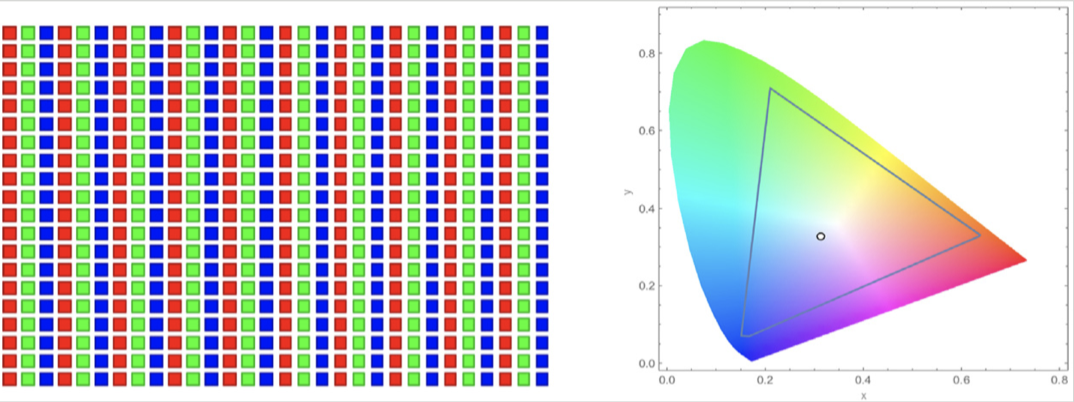
\includegraphics[width=0.9\textwidth]{figs/F2-a1.png}
\end{figure*}

DPC++ 中包含的一个附加选择器(SYCL 中不可用)
可通过包含标头“sycl/ext/intel/fpga\_extensions.hpp”来使用。

\begin{figure*}[!htbp]
	\centering
	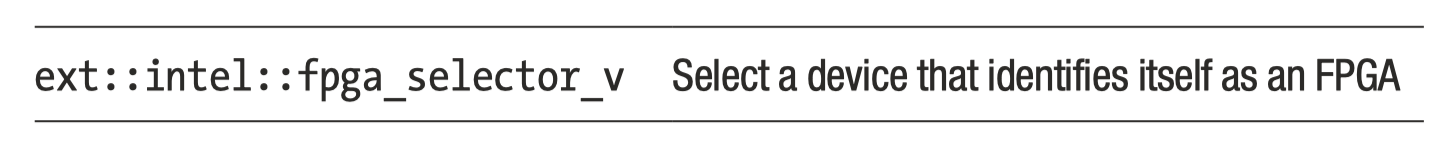
\includegraphics[width=0.9\textwidth]{figs/F2-a2.png}
\end{figure*}

可以使用内置选择器之一构造队列,例如

queue myQueue\{ gpu\_selector\_v\{\} \}; 

\begin{figure}[H]
	\centering
	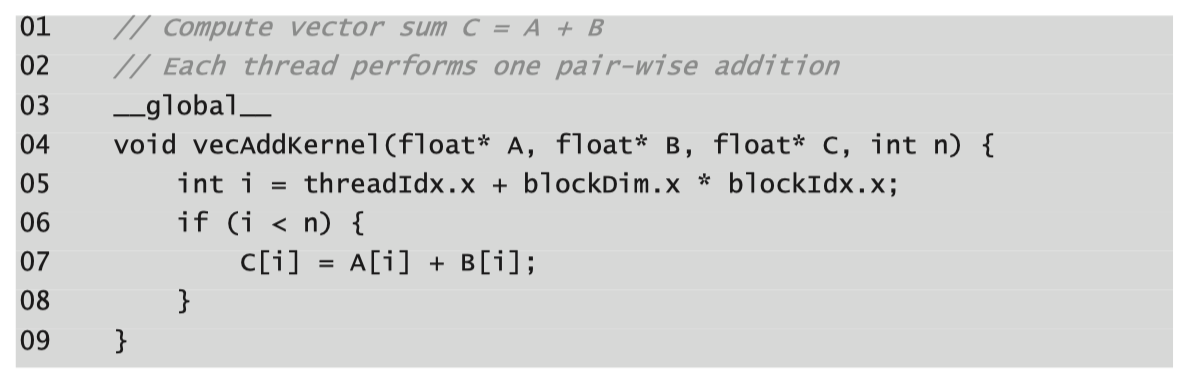
\includegraphics[width=0.9\textwidth]{figs/F2.10.png}
	\caption{\textit{GPU 设备选择器示例}}
\end{figure}

\begin{figure}[H]
	\centering
	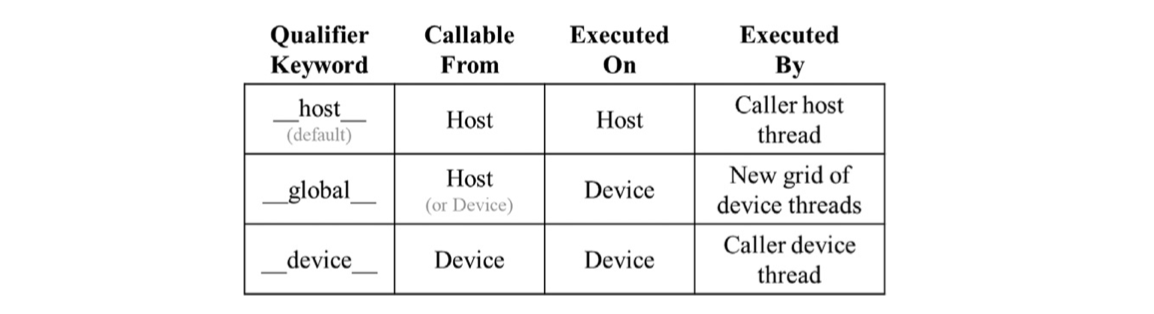
\includegraphics[width=0.9\textwidth]{figs/F2.11.png}
	\caption{\textit{绑定到应用程序可用的 GPU 设备的队列}}
\end{figure}

\begin{figure}[H]
	\centering
	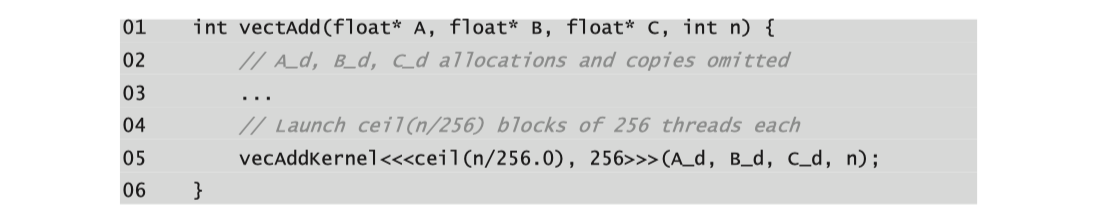
\includegraphics[width=0.9\textwidth]{figs/F2.12.png}
	\caption{\textit{来自各种类别的设备选择器的示例设备标识输出,
	并演示设备选择器不仅可用于构建队列(在本例中为构造设备类实例)}}
\end{figure}

图 2-10 显示了使用 GPU 选择器的完整示例,

图 2-11 显示了队列与可用 GPU 设备的相应绑定。

图 2-12 显示了使用各种内置选择器的示例,并演示了设备选择器与另一个在构造时接受设备选择器的类(设备)的使用。

\textbf{当设备选择失败时}

如果在创建对象(例如队列)时使用 GPU 选择器,并且没有可供运行时使用的 GPU 设备,则选择器将引发 runtime\_error 异常。 
对于所有设备选择器类都是如此,因为如果所需类的设备不可用,则会引发 runtime\_error 异常。 
对于复杂的应用程序来说,捕获该错误并获取不太理想的(对于应用程序/算法)设备类作为替代方案是合理的。 
第 5 章更详细地讨论了异常和错误处理。

\subsection{方法\#4:使用多个设备}
\begin{figure}[H]
	\centering
	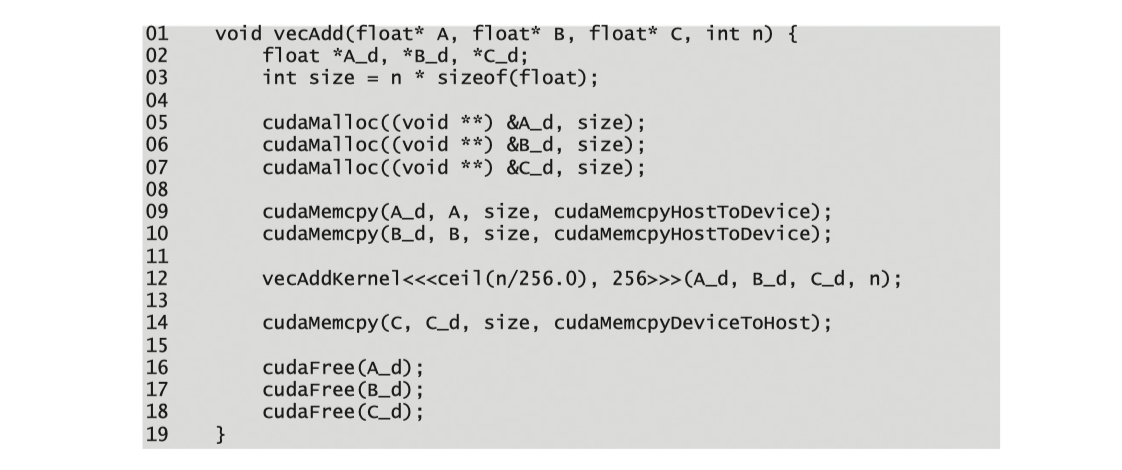
\includegraphics[width=0.9\textwidth]{figs/F2.13.png}
	\caption{\textit{为 GPU 和 FPGA 设备创建队列}}
\end{figure}

\begin{figure}[H]
	\centering
	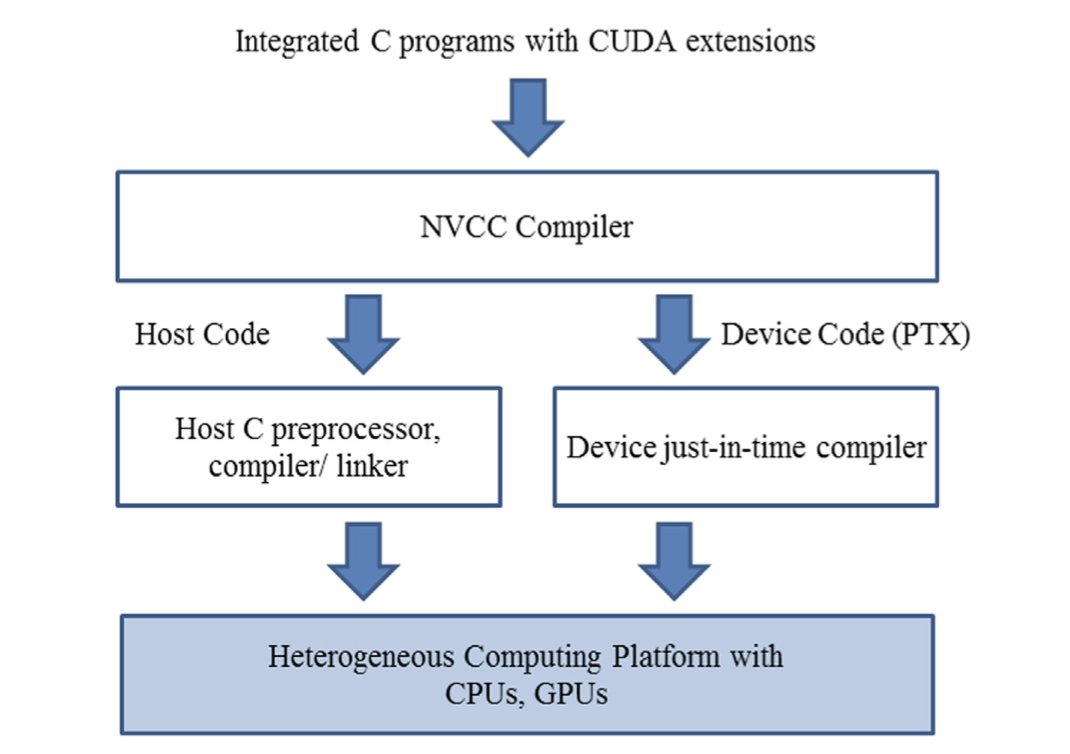
\includegraphics[width=0.9\textwidth]{figs/F2.14.png}
	\caption{\textit{GPU + FPGA 设备选择器示例:一个队列绑定到 GPU,另一个队列绑定到 FPGA}}
\end{figure}

如图2-5和2-6所示,我们可以在一个应用程序中构造多个队列。 
我们可以将这些队列绑定到单个设备(队列的工作总和集中到单个设备)、多个设备或这些设备的某种组合。 
图 2-13 提供了一个示例,创建一个绑定到 GPU 的队列和另一个绑定到 FPGA 的队列。 相应的映射如图 2-14 所示。

\subsection{方法\#5:自定义(非常具体)的设备选择}
现在我们将了解如何编写自定义选择器。 除了本章中的示例之外,第 12 章中还显示了更多示例。
内置设备选择器旨在让我们快速启动并运行代码。 
实际应用程序通常需要专门选择设备,例如从系统中可用的一组 GPU 类型中选择所需的 GPU。 
设备选择机制很容易扩展到任意复杂的逻辑,因此我们可以编写任何需要的代码来选择我们喜欢的设备。

\subsubsection{根据设备方面(Aspect)进行选择}
SYCL 定义了称为方面(Aspect)的设备属性。 
例如,设备可能展示的某些方面(在方面查询上返回 true)是 gpu、host\_debuggable、fp64 和 online\_compiler。 
请参阅 SYCL 规范的“设备方面”部分,了解标准方面及其定义的完整列表。

\begin{figure}[H]
	\centering
	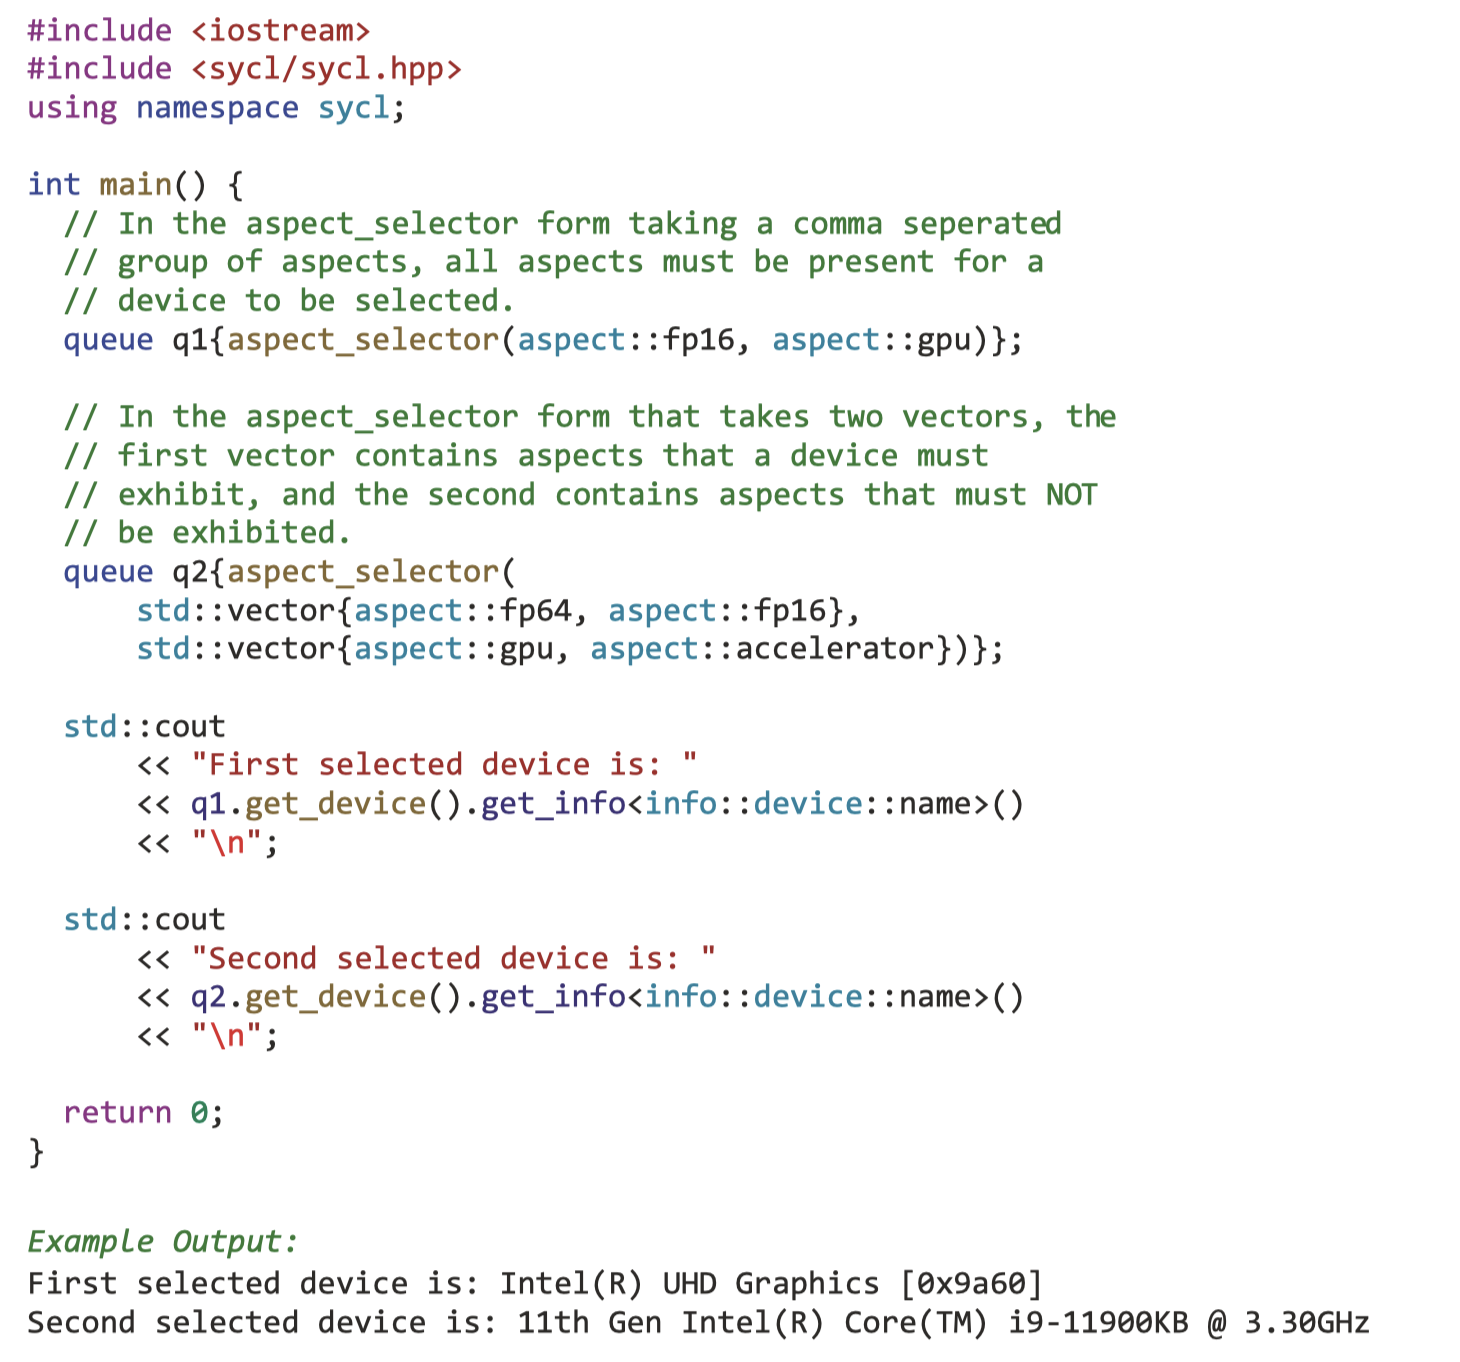
\includegraphics[width=0.9\textwidth]{figs/F2.15.png}
	\caption{\textit{Aspect selector}}
\end{figure}

要使用 SYCL 中定义的方面来选择设备,可以使用aspect\_selector,如图 2-15 所示。 
以aspect\_selector 的形式,采用逗号分隔的aspect 组,所有aspect 都必须由要选择的设备显示。 
spect\_selector 的另一种形式采用两个 std::vector。 
第一个向量包含设备中必须存在的方面,第二个向量包含设备中不得存在的方面(列出负面方面)。 
图2-15 显示了使用这两种形式的aspect\_selector 的示例。

一些方面可用于推断设备的性能特征。 例如,具有仿真方面的任何设备可能不如未仿真的相同类型的设备执行得那么好,
而是可以表现出与改进的可调试性相关的其他方面。

\subsubsection{通过自定义选择器进行选择}
当现有方面不足以选择特定设备时,可以定义自定义设备选择器。 
这样的选择器只是一个 C++ 可调用的(例如,函数或 lambda),
它接受 const Device\& 作为参数,并返回特定设备的整数分数。 
SYCL 运行时在可以找到的所有可用根设备上调用选择器,并选择选择器返回最高分数的设备(该分数必须为非负数才能进行选择)。

如果最高分数出现平局,SYCL 运行时将选择平局设备之一。 
运行时不会选择选择器返回负数的任何设备,因此从选择器返回负数可保证该设备不会被选择。

\textbf{设备评分机制}

我们有很多选项来创建与特定设备相对应的整数分数,例如:

\begin{enumerate}
	\item 返回特定设备类别的正值。

	\item 设备名称和/或设备供应商字符串的字符串匹配。

	\item 根据设备或平台查询,计算我们可以想象得到的任何整数值。
\end{enumerate}

\begin{figure}[H]
	\centering
	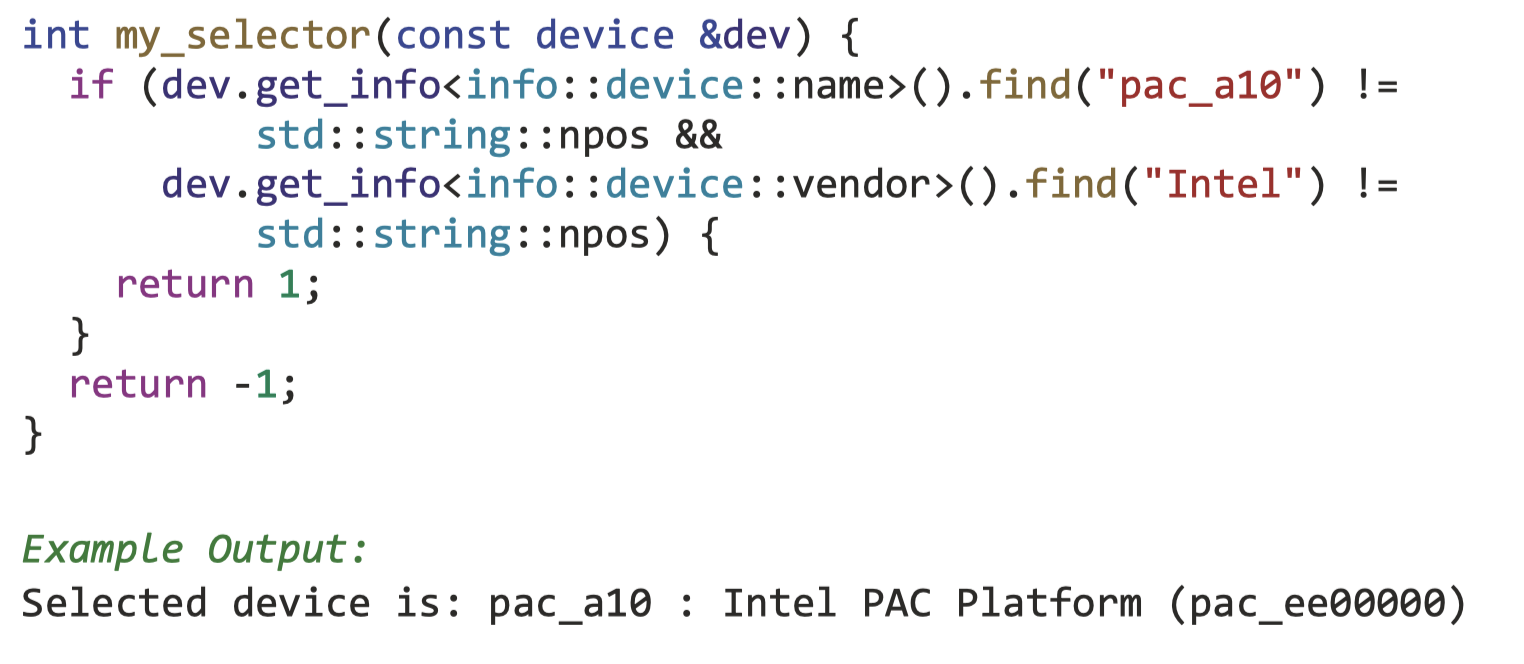
\includegraphics[width=0.9\textwidth]{figs/F2.16.png}
	\caption{\textit{特定英特尔 Arria FPGA 加速板的自定义选择器}}
\end{figure}

例如,选择特定 Intel Arria FPGA 加速器板的一种可能方法如图 2-16 所示。

第12章有更多关于设备选择的讨论和示例,并更深入地讨论了get\_info方法。

\subsection{在设备上创建任务}
应用程序通常包含主机代码和设备代码的组合。 有一些类成员允许我们提交设备代码以供执行,
并且由于这些工作调度构造是提交设备代码的唯一方法,因此它们使我们能够轻松区分设备代码和主机代码。

本章的其余部分介绍了一些工作调度结构,目的是帮助我们理解和识别设备代码和在主机处理器上本机执行的主机代码之间的划分。

\subsubsection{任务图简介}
\begin{figure}[H]
	\centering
	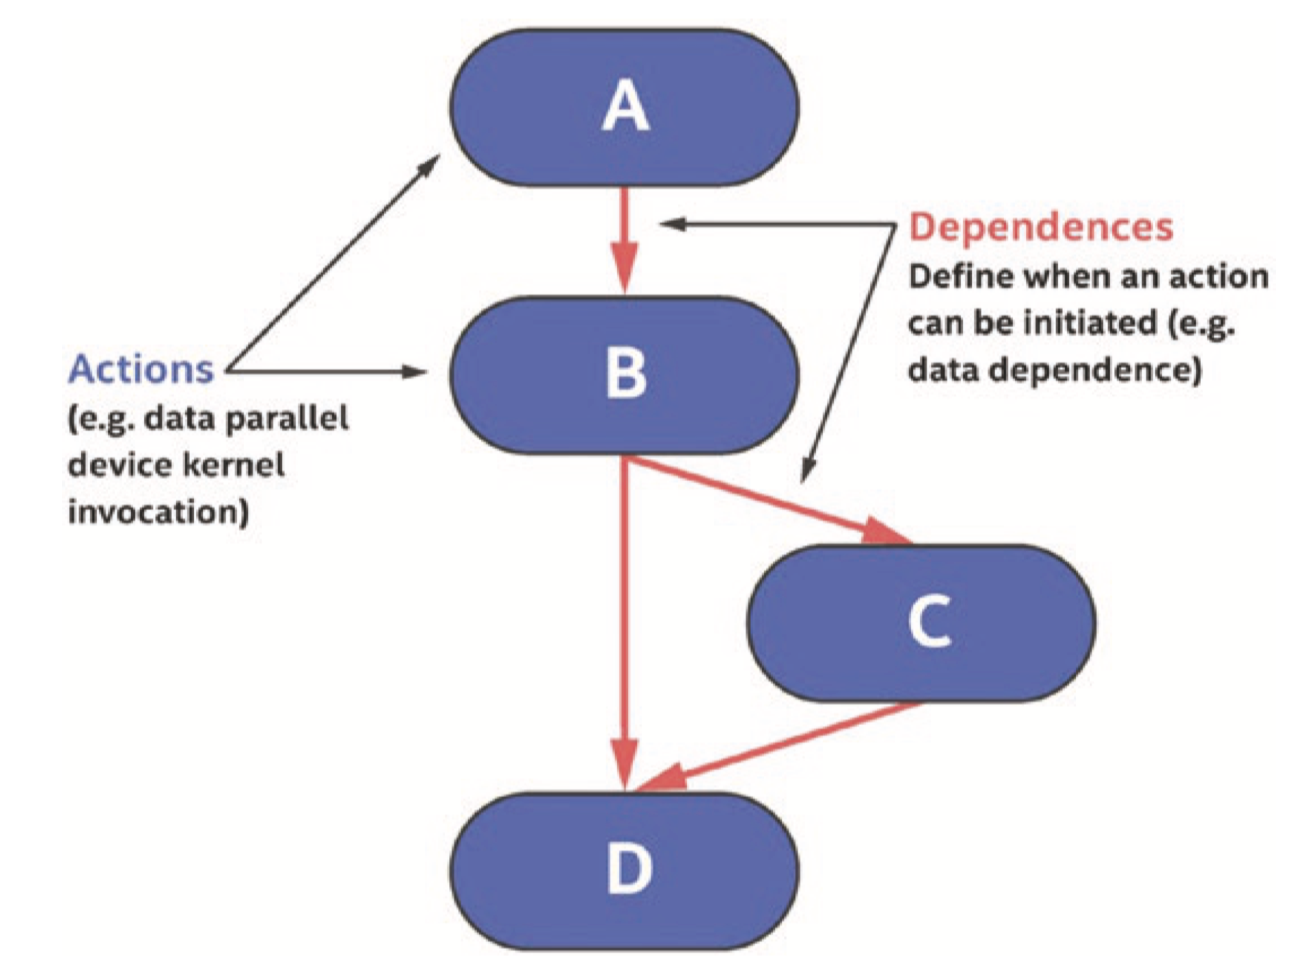
\includegraphics[width=0.9\textwidth]{figs/F2.17.png}
	\caption{\textit{任务图定义要在一个或多个设备上执行的操作(从主机程序异步执行),
	以及确定操作何时可以安全执行的依赖关系}}
\end{figure}

SYCL 执行模型中的一个基本概念是节点图。 该图中的每个节点(工作单元)都包含要在设备上执行的动作,
最常见的动作是数据并行设备Kernel调用。 图 2-17 显示了具有四个节点的示例图,其中每个节点都可以被视为设备Kernel调用。

图 2-17 中的节点具有依赖边,定义节点的工作何时开始执行是合法的。 
依赖边通常是根据数据依赖自动生成的,尽管我们可以通过一些方法在需要时手动添加额外的自定义依赖。 
例如,图中的节点 B 具有来自节点 A 的依赖边。该边意味着节点 A 必须完成执行,
并且很可能(取决于依赖关系的具体情况)使生成的数据在节点 B 将执行的设备上可用 在节点B的动作开始之前。 
运行时控制依赖关系的解析和节点执行的触发,与主机程序的执行完全异步。 
定义应用程序的节点图在本书中将称为任务图,并在第 3 章中进行更详细的介绍。

\subsubsection{设备代码在哪里?}
有多种机制可用于定义将在设备上执行的代码,但一个简单的示例展示了如何识别此类代码。 
即使示例中的模式乍一看很复杂,但该模式在所有设备代码定义中保持相同,因此很快就成为第二天性。

\begin{figure}[H]
	\centering
	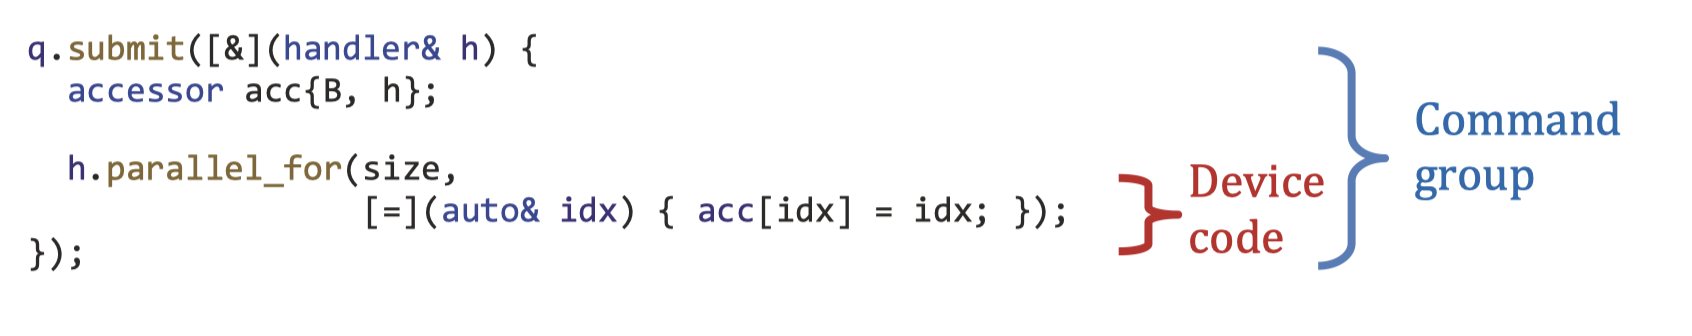
\includegraphics[width=0.9\textwidth]{figs/F2.18.png}
	\caption{\textit{提交设备代码}}
\end{figure}

作为最后一个参数传递给parallel\_for 的代码(定义为图2-18 中的lambda 表达式)是要在设备上执行的设备代码。 
在这种情况下,parallel\_for 是让我们区分设备代码和主机代码的构造。 
parallel\_for 是一小组设备调度机制之一,所有成员都是处理程序类,定义要在设备上执行的代码。 
图 2-19 给出了处理程序类的简化定义。

\begin{figure}[H]
	\centering
	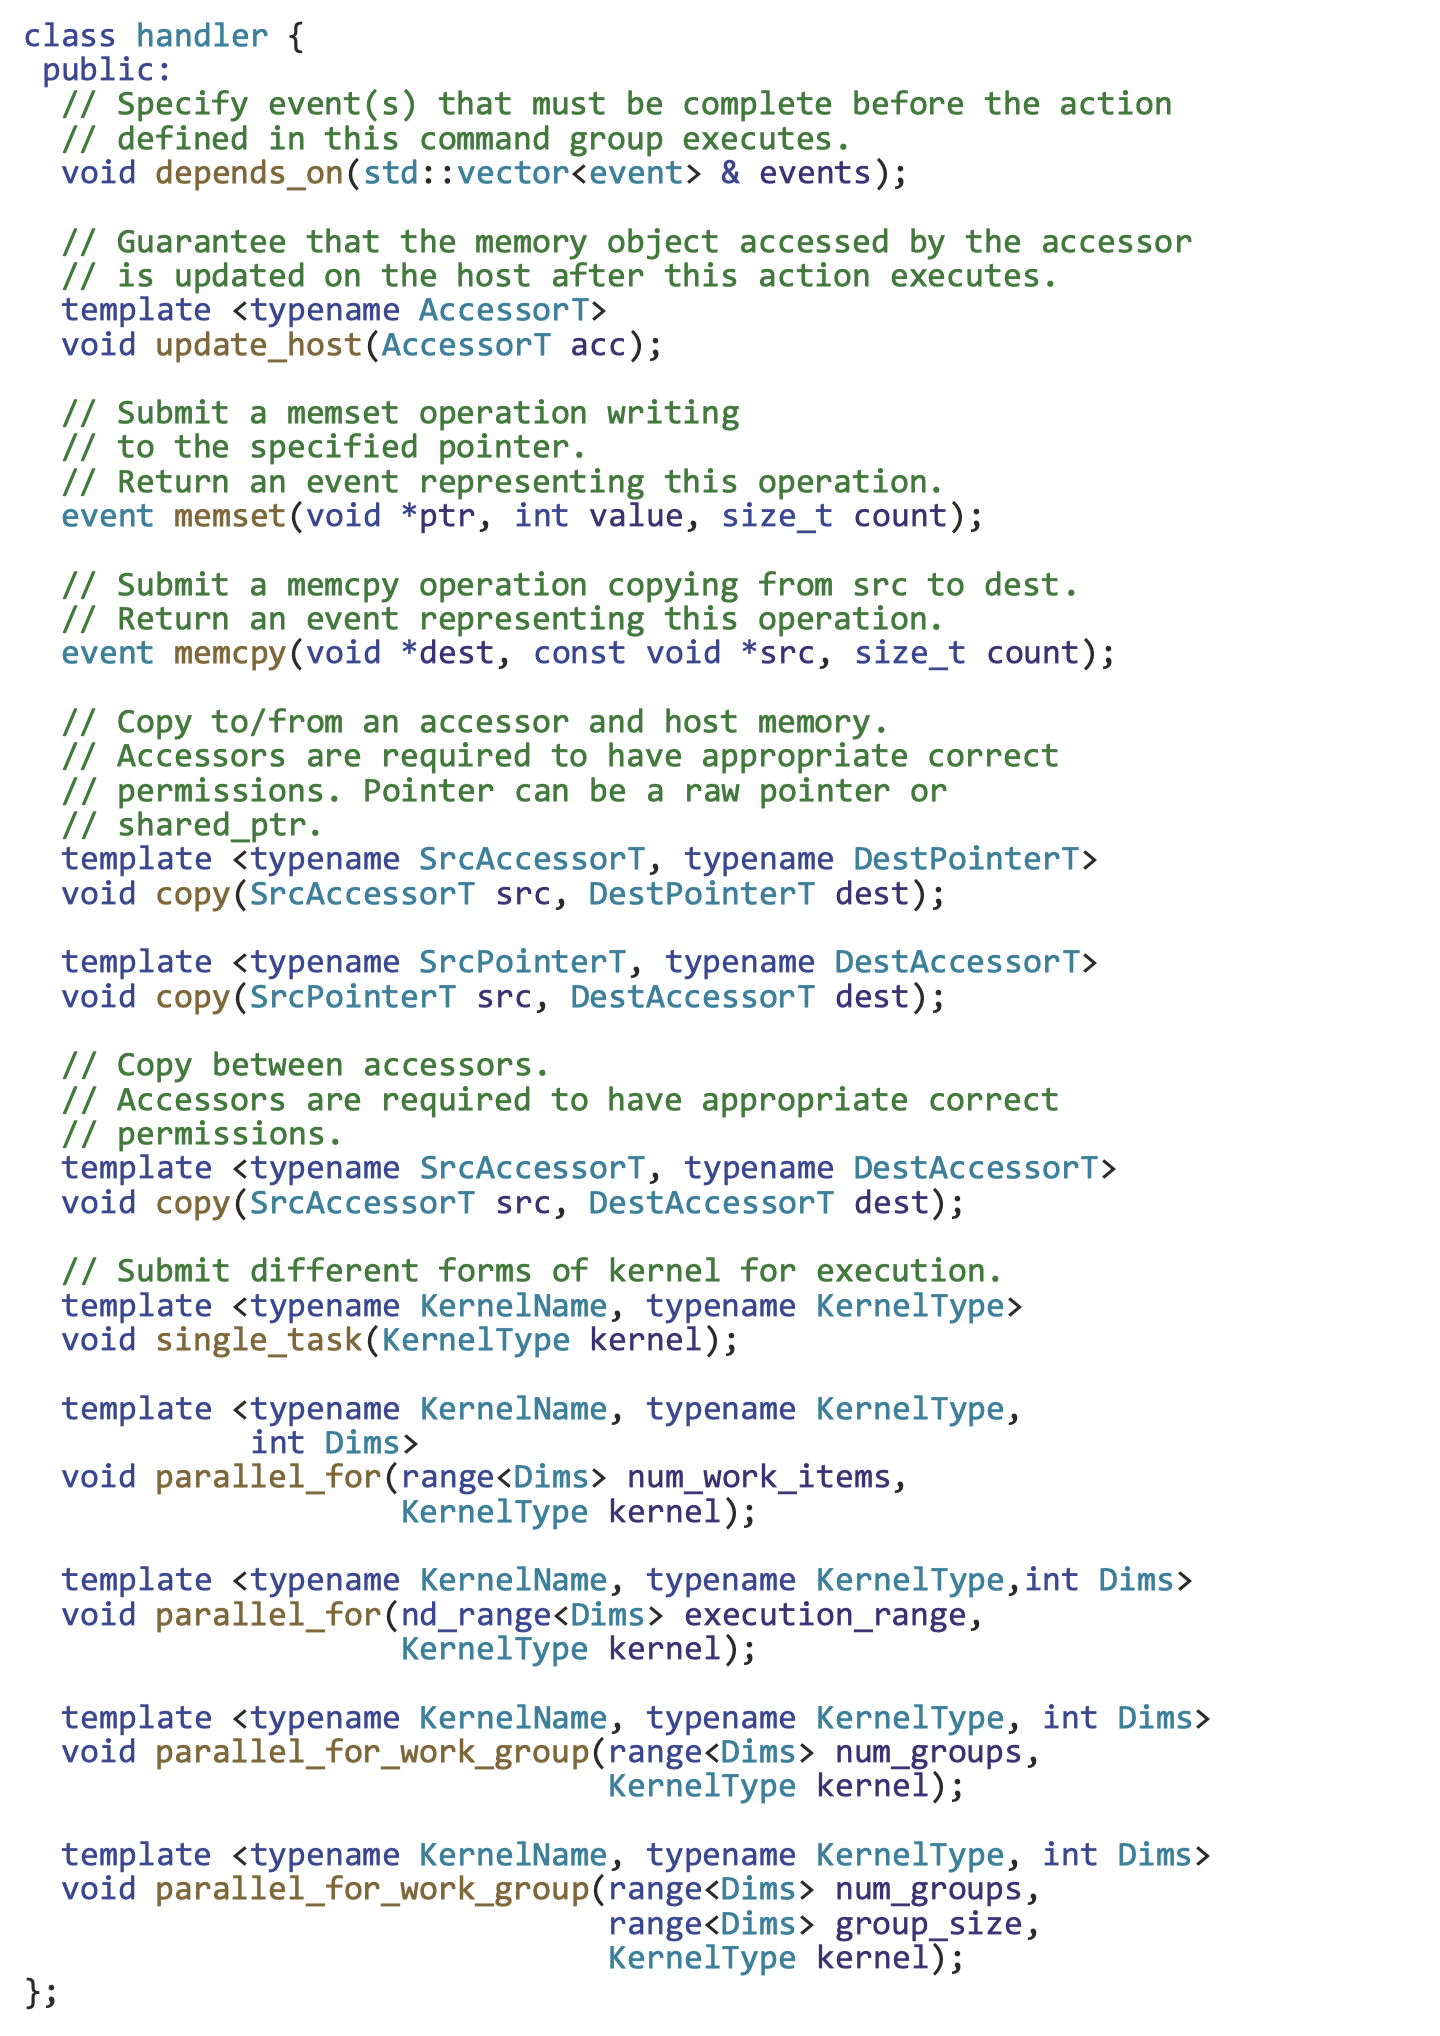
\includegraphics[width=0.9\textwidth]{figs/F2.19.png}
	\caption{\textit{处理程序类中成员函数的简化定义}}
\end{figure}

\begin{figure}[H]
	\centering
	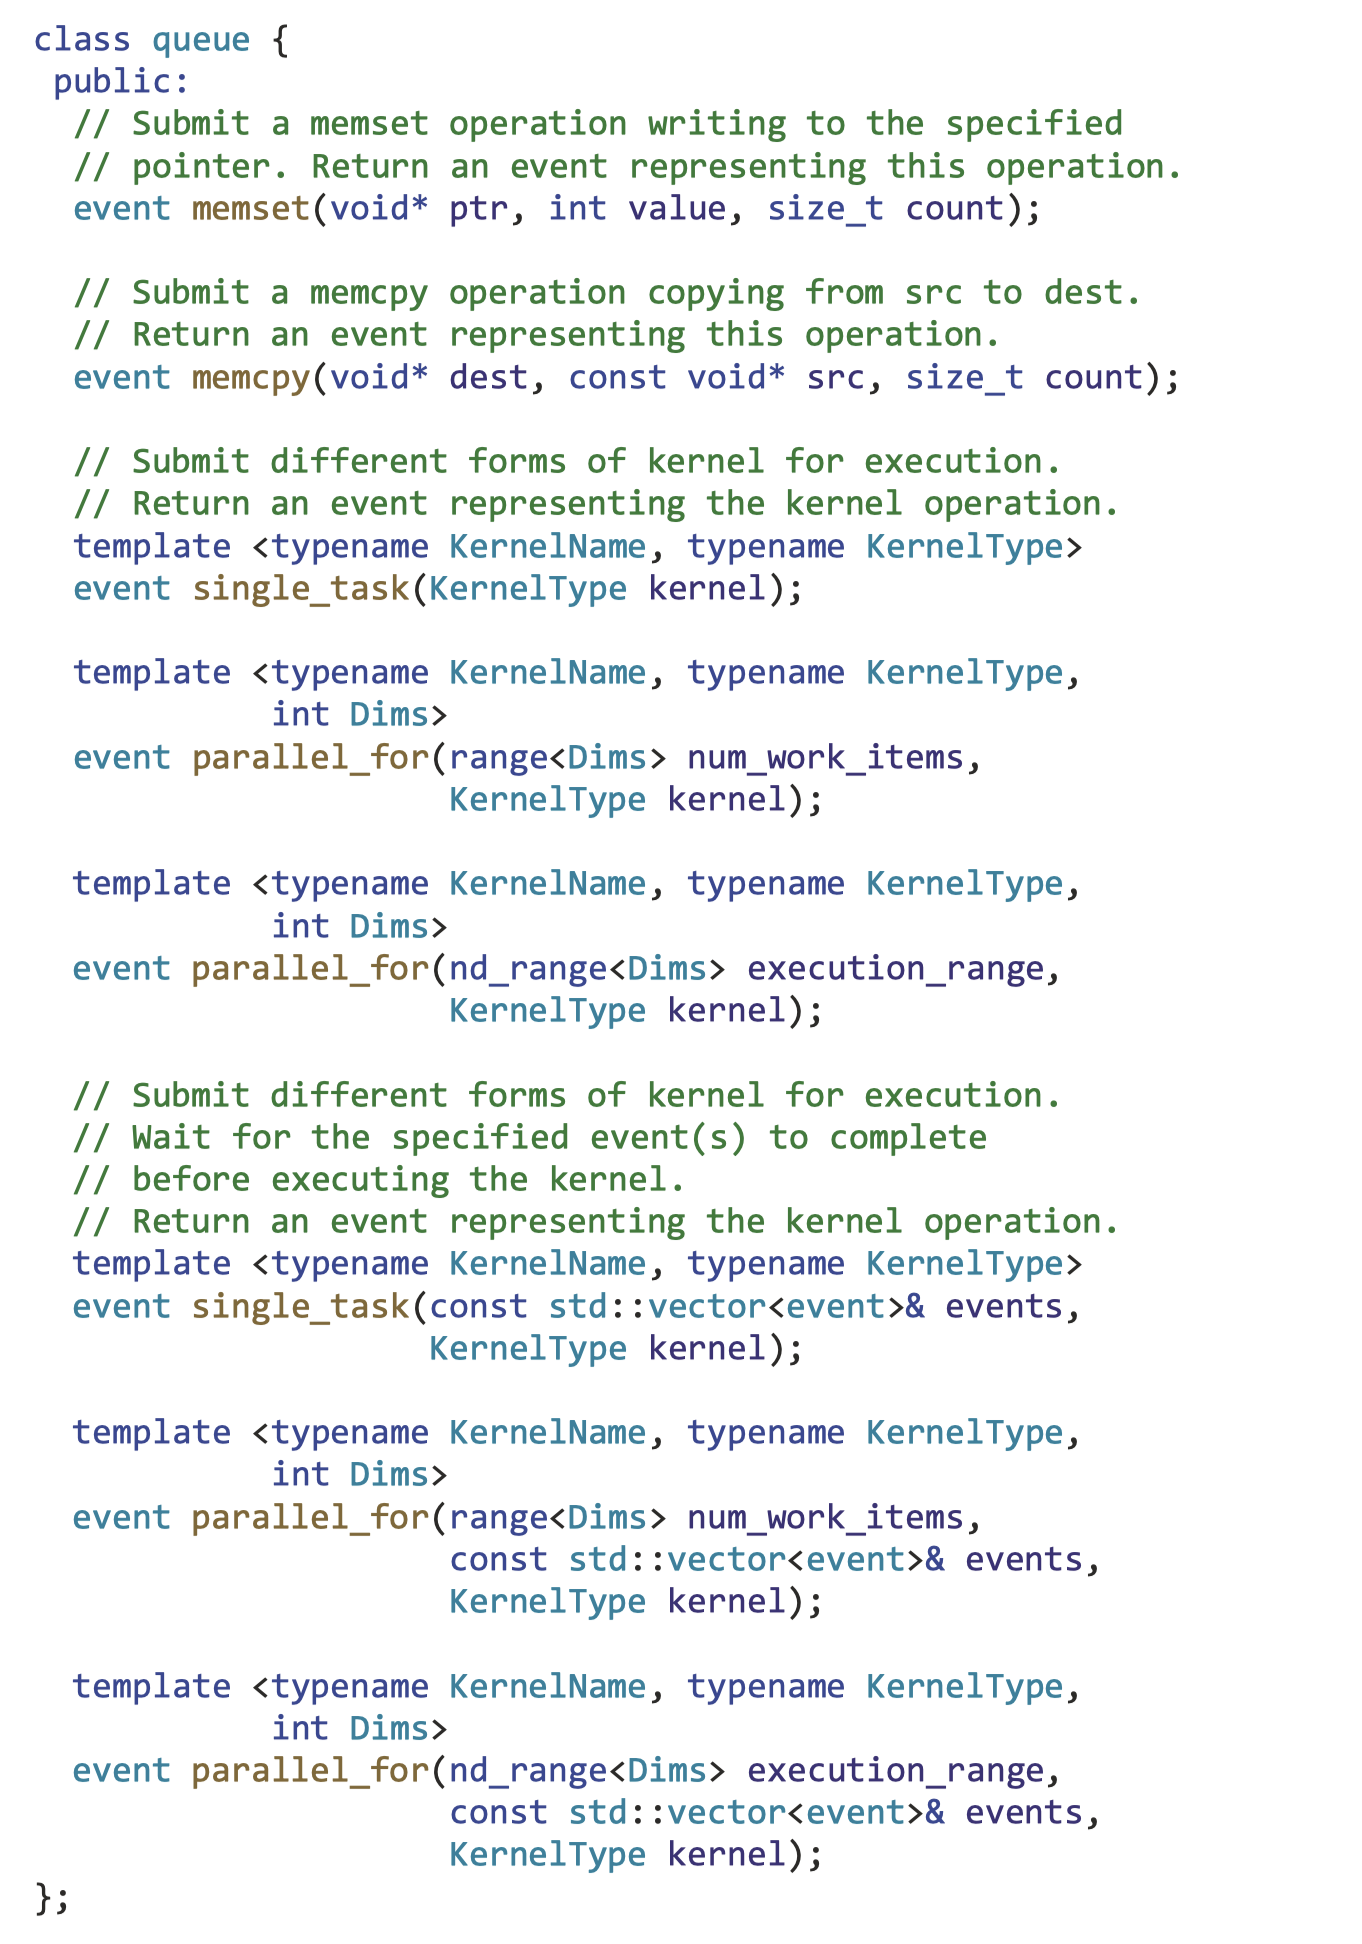
\includegraphics[width=0.9\textwidth]{figs/F2.20.png}
	\caption{\textit{简化了队列类中成员函数的定义,这些函数充当处理程序类中等效函数的简写表示法}}
\end{figure}

除了调用处理程序类的成员来提交设备代码之外,还有队列类的成员允许提交工作。 
图 2-20 中所示的队列类成员是简化某些模式的快捷方式,我们将在以后的章节中看到这些快捷方式的使用。

\subsubsection{行动}
图2-18中的代码包含一个parallel\_for,它定义了要在设备上执行的工作。 
Parallel\_for 位于提交给队列的命令组 (CG) 内,队列定义要在其上执行工作的设备。 在命令组内,有两类代码:

\begin{enumerate}
	\item 设置依赖关系的主机代码,定义运行时何时可以安全地开始执行 (2) 中定义的工作,
	例如创建缓冲区访问器(第 3 章中描述)

	\item 最多调用一次对设备代码进行排队以供执行或执行手动内存动作(例如复制)的动作
\end{enumerate}

处理程序类包含一小组成员函数,这些函数定义执行任务图节点时要执行的动作。 图 2-21 总结了这些动作。

\begin{figure}[H]
	\centering
	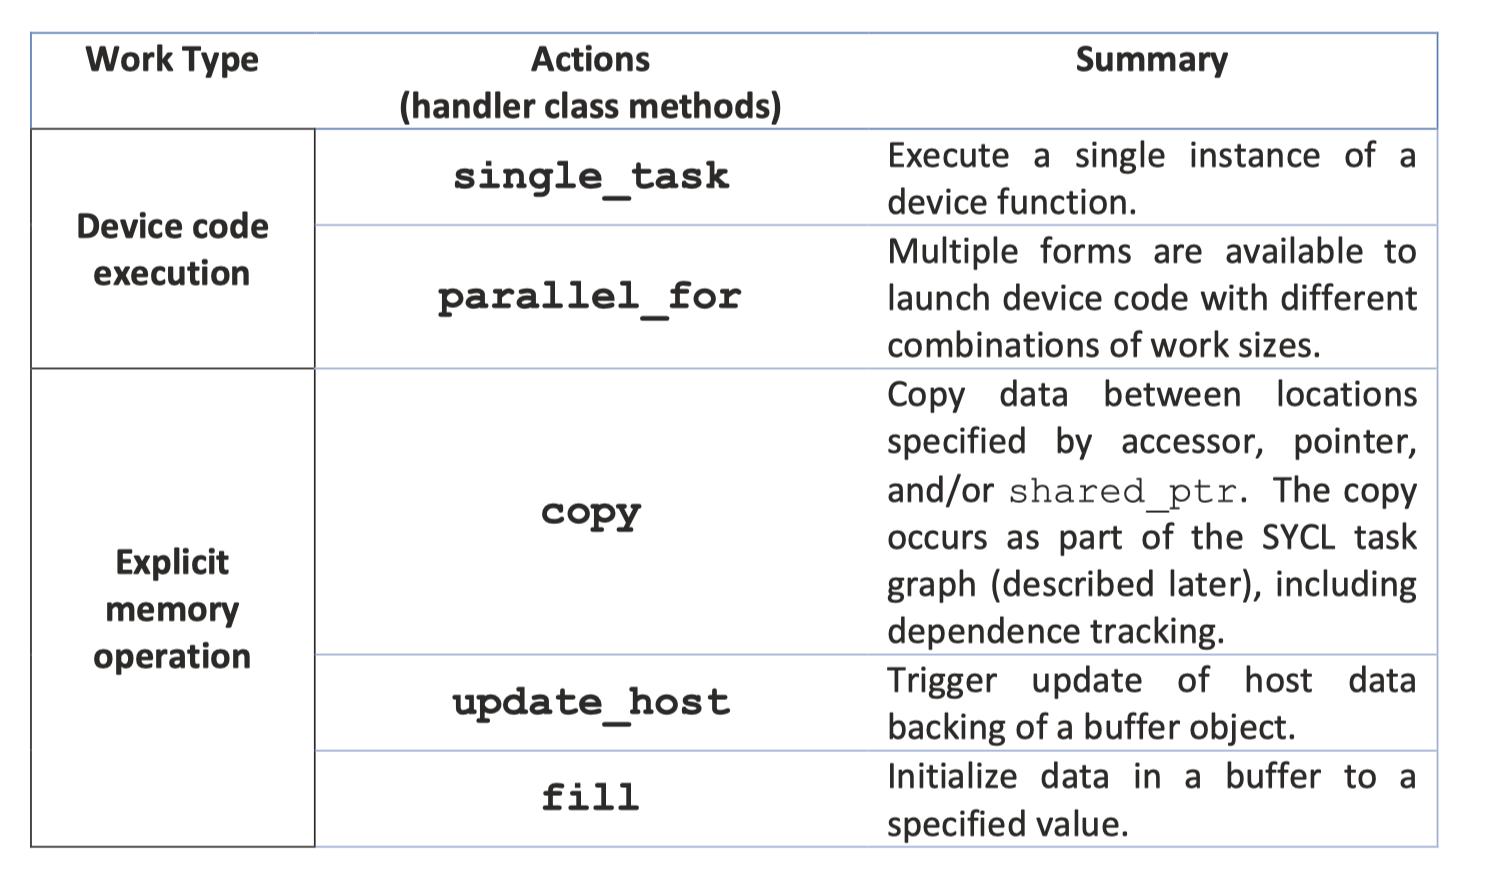
\includegraphics[width=0.9\textwidth]{figs/F2.21.png}
	\caption{\textit{触发设备代码,以及显式的内存操作}}
\end{figure}

一个命令组内最多可以调用图 2-21 中的一个动作(调用多个动作是错误的),并且每个提交调用只能将一个命令组提交到队列中。 
其结果是,每个任务图节点都存在图 2-21 中的单个(或可能没有)动作,
该动作将在满足节点依赖性并且运行时确定可以安全执行时执行。

\begin{remark}
命令组中最多只能有一个操作,例如Kernel启动或显式内存操作。
\end{remark}

代码在未来异步执行的想法是作为主机程序的一部分在 CPU 上运行的代码与将来在满足依赖性时运行的设备代码之间的关键区别。 
命令组通常包含每个类别的代码,其中定义依赖关系的代码作为主机程序的一部分运行(以便运行时知道依赖关系是什么),
而设备代码则在满足依赖关系后运行。

\begin{figure}[H]
	\centering
	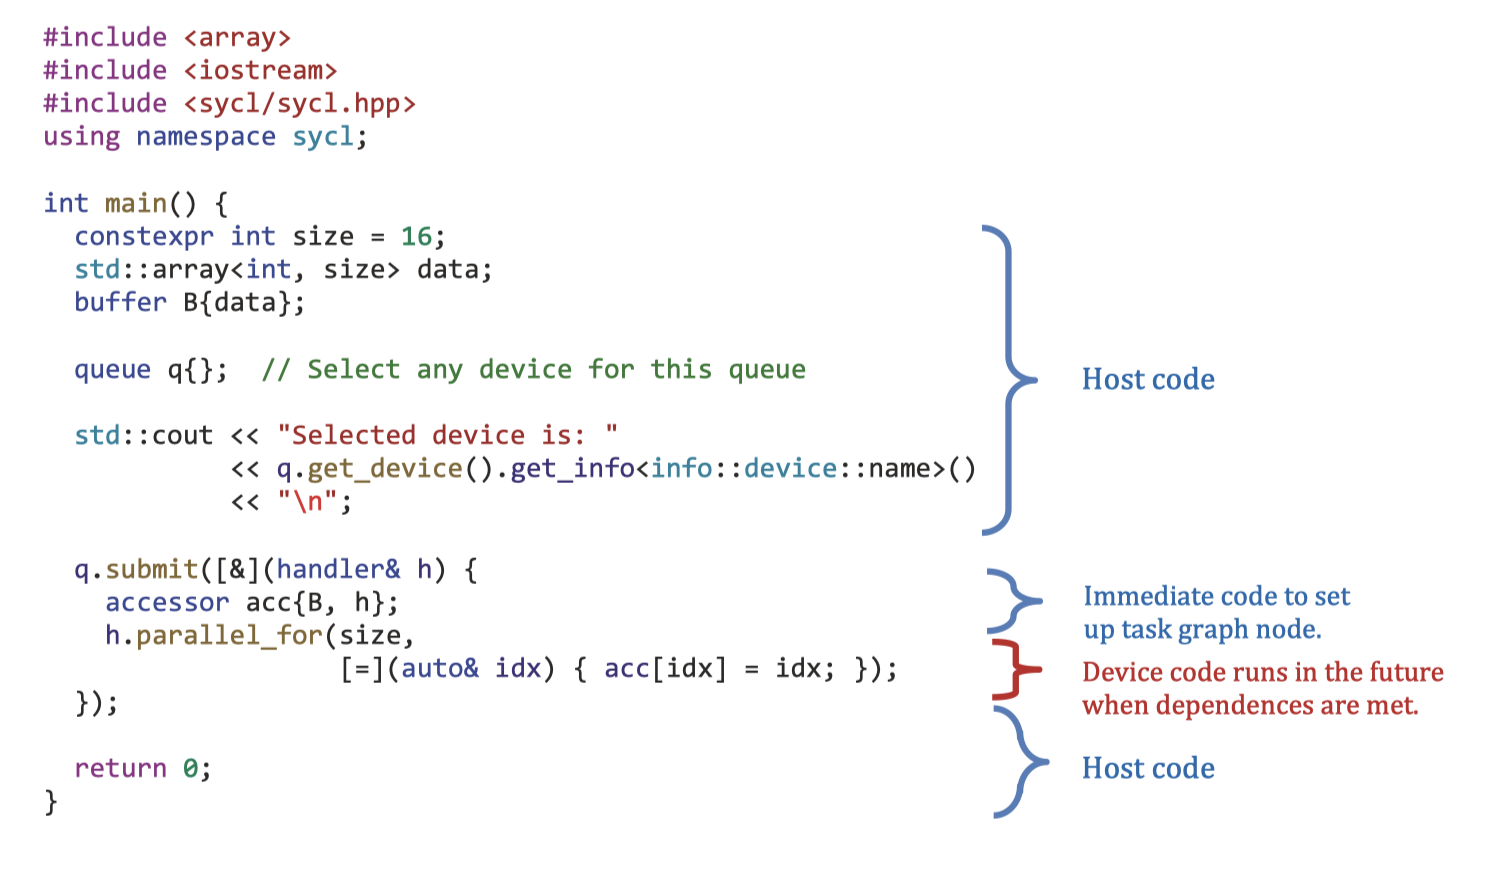
\includegraphics[width=0.9\textwidth]{figs/F2.22.png}
	\caption{\textit{提交设备代码}}
\end{figure}

图 2-22 中有三类代码:

\begin{enumerate}
	\item 主机代码:驱动应用程序,包括创建和管理数据缓冲区以及将工作提交到队列以在任务图中形成新节点以进行异步执行。

	\item 命令组内的主机代码:此代码在执行主机代码的处理器上运行,并在提交调用返回之前立即执行。 
	例如,此代码通过创建访问器来设置节点依赖性。 
	任何任意 CPU 代码都可以在这里执行,但最佳实践是将其限制为配置节点依赖项的代码。

	\item 动作:图2-21中列出的任何动作都可以包含在命令组中,它定义了将来满足节点要求时异步执行的工作(由(2)设置)。
\end{enumerate}

要了解应用程序中的代码何时运行,请注意,传递给图 2-21 中列出的启动设备代码执行的动作的任何内容,
或图 2-21 中列出的显式内存动作,将来当 SYCL 任务图(稍后描述)节点依赖性已得到满足。 
所有其他代码立即作为主机程序的一部分运行,正如典型 C++ 代码中所预期的那样。

需要注意的是,虽然设备代码可以在满足任务图节点依赖性时开始(异步)运行,但不能保证设备代码在此时开始运行。 
确保设备代码开始执行的唯一方法是让主机程序通过主机访问器或队列等待动作等机制等待(阻塞)设备代码执行的结果,
我们将在后面的章节中介绍这些机制。 如果没有此类主机阻塞动作,SYCL 和较低级别的运行时将决定何时开始执行设备代码,
可能会针对“尽快运行”以外的目标进行优化,例如针对功耗或拥塞进行优化。

\subsubsection{主机任务}
一般来说,提交到队列(例如通过parallel\_for)的动作执行的代码是设备代码,遵循一些语言限制,
使其能够在许多体系结构上高效运行。 不过,有一个重要的偏差是通过名为 host\_task 的处理程序方法访问的。 
此方法允许将任意 C++ 代码作为任务图中的动作提交,并在满足任何任务图依赖性后在主机上执行。

主机任务在某些程序中很重要,原因有二:
\begin{enumerate}
	\item 可以包含任意C++,甚至std::cout或printf。 
	这对于轻松调试、与 OpenCL 等较低级别 API 的互动作性或在现有代码中逐步启用加速器非常重要。

	\item 主机任务作为任务图的一部分异步执行,而不是与主机程序同步执行。 
	尽管主机程序可以启动附加线程或使用其他任务并行方法,但主机任务与 SYCL 运行时的依赖性跟踪机制集成。 
	当设备和主机代码需要分散时,这非常方便,并且可能会带来更高的性能。
\end{enumerate}

\begin{figure}[H]
	\centering
	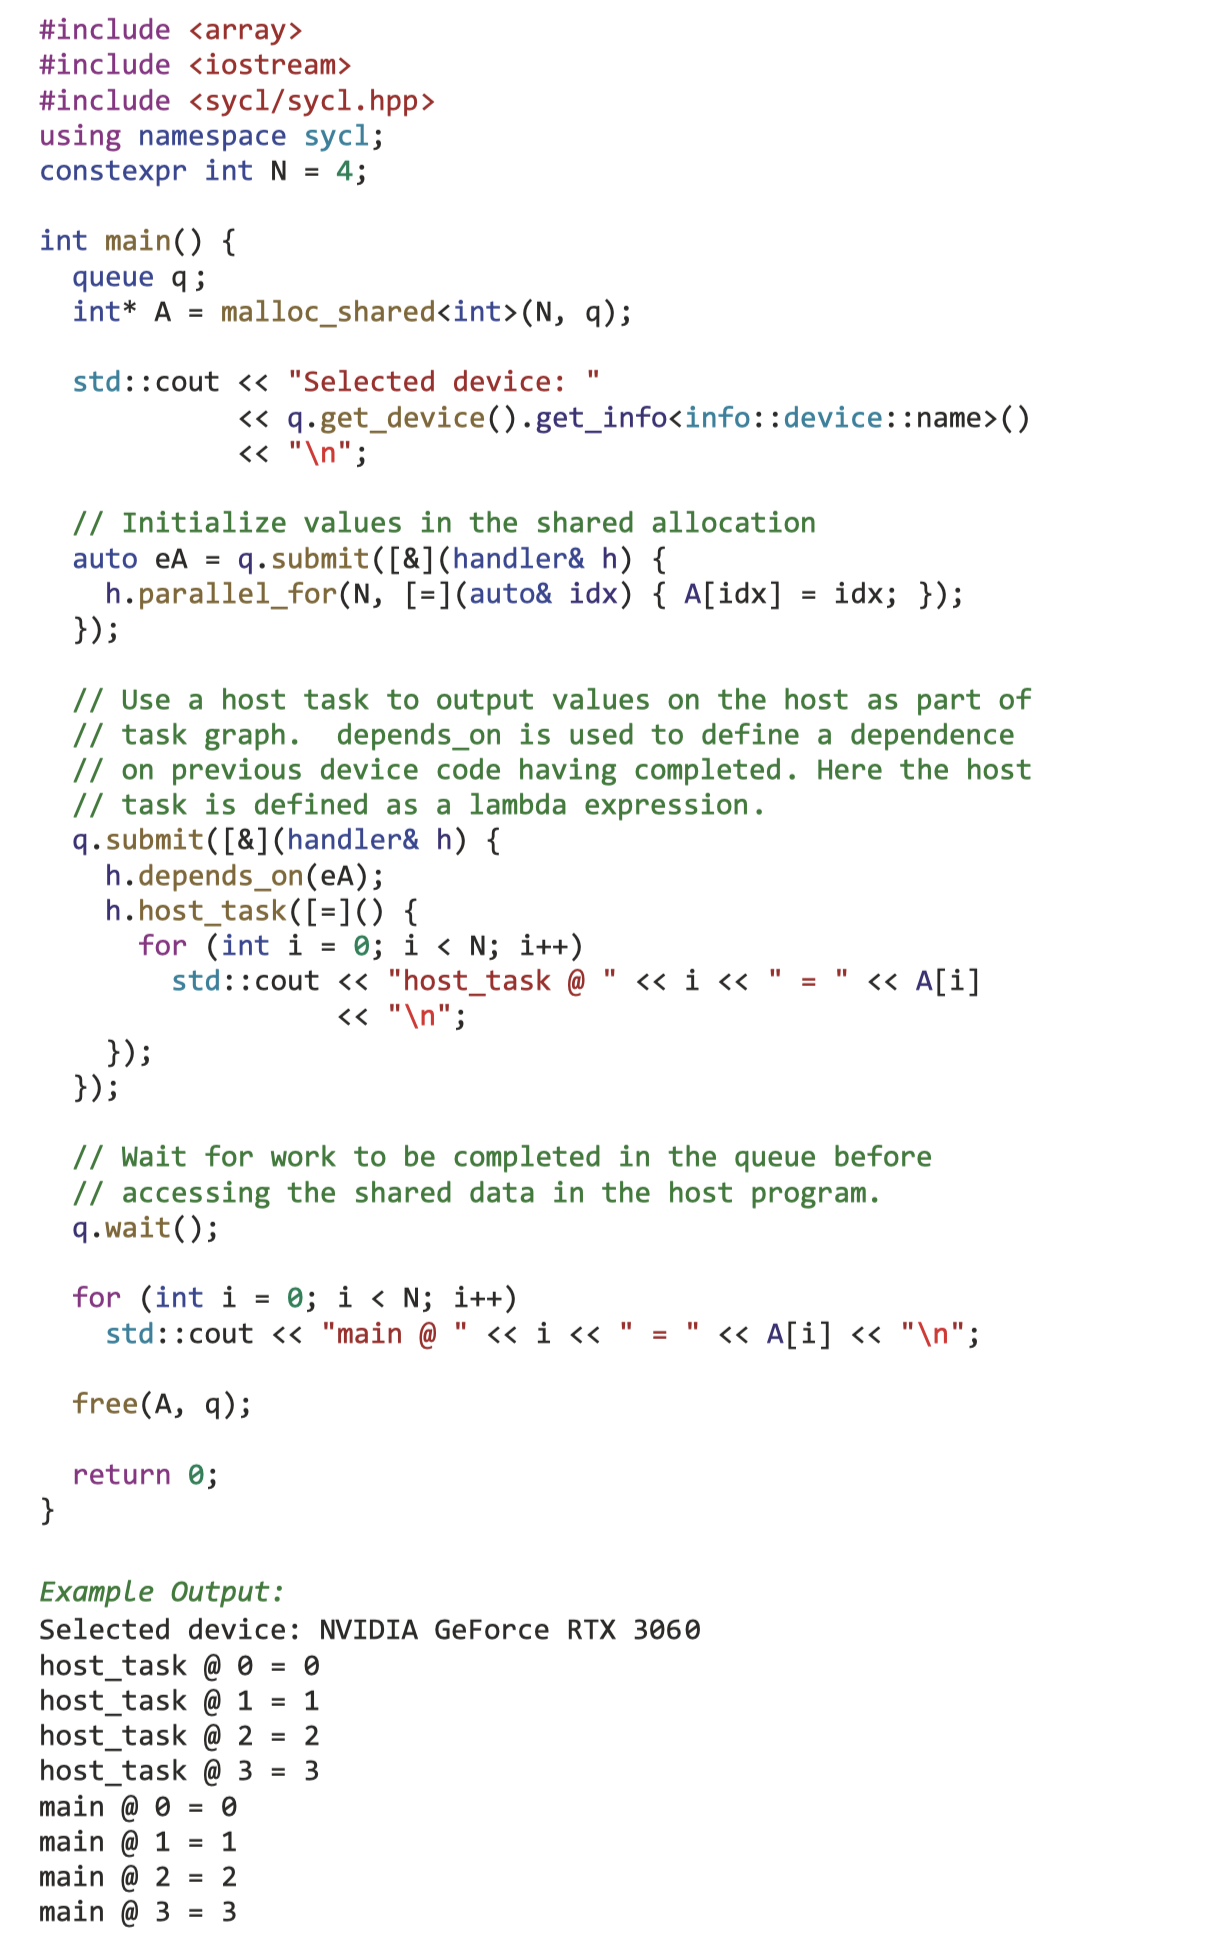
\includegraphics[width=0.9\textwidth]{figs/F2.23.png}
	\caption{\textit{简单的host\_task 例子}}
\end{figure}

图 2-23 演示了一个简单的主机任务,当满足任务图依赖性时,它使用 std::cout 输出文本。 
请记住,主机任务是与主机程序的其余部分异步执行的。 
这是任务图机制的强大部分,其中 SYCL 运行时在安全时安排工作,而无需与主机程序交互,而主机程序可能会继续其他工作。

另请注意,主机任务的代码主体不需要遵循对设备代码施加的任何限制(如第 10 章所述)。

图 2-23 中的示例基于事件(在第 3 章中描述)来创建设备代码提交和后续主机任务之间的依赖关系,
但是主机任务也可以通过以下方式与访问器(也在第 3 章中介绍)
一起使用: target::host\_task 的特殊访问器模板参数化(第 7 章)。

\subsection{总结}
在本章中,我们概述了队列、与队列关联的设备的选择以及如何创建自定义设备选择器。 
我们还概述了满足依赖性时在设备上异步执行的代码与作为 C++ 应用程序主机代码的一部分执行的代码。 
第 3 章介绍如何控制数据移动。